\documentclass{article}
\usepackage[utf8]{inputenc}
\usepackage[norsk]{babel} 
\usepackage{listings}
\usepackage[sfdefault,light]{roboto}  %font
\usepackage[T1]{fontenc} %font
\usepackage{graphicx} %images
\usepackage[table,xcdraw]{xcolor} %color in tables
\usepackage{array} %tabular: allow multiple lines
\usepackage{longtable} %table that can go over multiple lines
\usepackage{amsfonts} %checkmark
\usepackage{float} %force position
\usepackage{booktabs}
\newcommand{\tabitem}{~~\llap{\textbullet}~~}
\usepackage{setspace}%line spacing
\onehalfspacing

%\usepackage{multicol} %allows for multicolumn itemize

\usepackage{geometry} %size of paper
 \geometry{
 a4paper,
 total={170mm,257mm},
 left=25mm,
 right=25mm,
 top=25mm,
 bottom=25mm,
 }

\newcolumntype{L}[1]{>{\raggedright\let\newline\\\arraybackslash}m{#1}} %better looking multirow cells

\begin{document}
\begin{center}
\vspace*{4.5cm}
\Huge{Prosjektrapport}\\[2pc]
\vspace{-1.5cm}
\noindent\rule{11cm}{0.8pt}\\

\Large{IT3402: Design av grafiske brukergrensesnitt}\\[1pc]
\vspace{-0.7cm}
\noindent\rule{11cm}{0.8pt}\\
\vspace{3.5cm}

\large{{\textbf{Gruppe 15}: \\
Martin Dørum\\
Andrea Leikvold\\
Signe Elise Livgard\\
Anne-Marie Samuelsen\\
}}
\vspace{2.0cm}

\large{28. November 2016}\\
\vspace{1.0cm}

\includegraphics[scale=0.6]{images/ntnu.png}
\end{center}

\setlength{\parindent}{4em}
\setlength{\parskip}{1em} % space between index lines
\renewcommand{\baselinestretch}{1.3} % space between lines

\thispagestyle{empty}
\newpage
\thispagestyle{empty}
\begin{center}
Denne siden er ment å være blank.
\end{center}
\null\newpage
\setcounter{page}{1}
\pagenumbering{roman}

\tableofcontents
\newpage
\listoftables
\newpage
\listoffigures
\newpage

\setcounter{page}{1}
\pagenumbering{arabic}

\section{\textcolor[HTML]{D32F2F}{Introduksjon}}
Denne rapporten er skrevet som et resultat av arbeidet gjort i emnet \textit{IT3402: Design av grafiske brukergrensesnitt} ved Norges Teknisk-Naturvitenskapelige Universitet, høsten 2016. Emnet inngår som et obligatorisk emne for studenter tatt opp på masterstudiet i informatikk, i retningen \textit{Interaksjonsdesign, spill og læringsteknologi}.
\\\\
Temaet for oppgaven gitt i emnet var kjøpesentre, og gruppene ble bedt om å lage en app for å løse kunders behov rundt handleopplevelsen på et senter. Kjøpesentrene var lokalisert i Trondheim. 
\\\\
Målet med oppgaven har vært å forstå brukernes ønsker og de mulighetene som teknologien gir til brukervennlige og nyttige produkter og tjenester. Det var ikke noe mål om å komme opp med den mest oppsiktsvekkende eller nytenkende løsningen, men heller ha fokus på å lære brukersentrert design i praksis.
\newpage

\section{\textcolor[HTML]{D32F2F}{Oppgaven}}

\subsection{Problembeskrivelse}
Gruppen fikk i oppgave å kartlegge behovet for en app på Sirkus Shopping, et kjøpesenter i Trondheim. Gruppen skulle gå gjennom hele prosessen, fra observasjoner og intervjuer, til prototyping, testing og utvikling av et ferdig produkt. Fokuset skulle ligge på brukersentrert design og iterative prosesser. 
\\\\
Sirkus shopping er et kjøpesenter på Persaunet i Trondheim. Her er det rundt 100 butikker, samt mange parkeringsplasser og lett tilgjengelighet med kollektivtransport. Målgruppen for kjøpesenteret er småbarnsforeldre og studenter, noe som gjenspeiles i butikkene på senteret.  Her finner man alt fra bokhandel, babybutikker og gullsmed til leketøysbutikk og hudklinikk\cite{sirkus}. Logoen til kjøpesenteret er vist i Figur \ref{fig:sirkus}.

\begin{figure}[H]

\includegraphics[scale=0.6]{images/sirkus}
\centering %centering the image
\caption{Logo Sirkus shopping}
\label{fig:sirkus}
\end{figure}

\subsection{Kravspesifikasjon}
Prosjektoppgaven gruppen fikk presentert omhandlet å forbedre shoppingopplevelsen. Oppgaven gikk ut på å bruke den nye generasjonen mobiltelefoner på nye måter. Her var iPhone og Android trukket fram som eksempler, hvor man skulle finne en måte å bruke teknologien i sammenheng med alt man gjør på et handlesenter. Målgruppen var kunder på et kjøpesenter, hvor hver gruppe fikk tildelt et spesifikt senter. Her skulle gruppen observere og intervjue målgruppen, og gjennom dette finne ut hva de kunne ønske seg på en smarttelefon. Dette skulle gruppen så lage en prototype av, og teste på faktiske brukere.
\\\\
I oppgaveteksten ble det oppfordret til å koble produktet opp mot sosiale medier, som for eksempel Twitter eller Facebook. Det ble også oppfordret til å bruke annen teknologi, som for eksempel smartklokker som Apple Watch. 
\\\\
Det ble gitt flere retningslinjer for løsningen gruppen skulle lage. De fire viktigste kravene var brukbarhet, selvmotivasjon, innhold og dialog. I brukbarhet ligger det at produktet skal være selvforklarende og intuitivt å bruke. I selvmotivasjon ligger det at produktet skal være laget slik at desto mer tid brukeren bruker sammen med produktet, eller i appen, desto mer lyst skal brukeren ha til å bruke produktet. Innholdet i produktet skulle gi korrekt informasjon, slik at kunden kunne stole på det produktet ga av opplysninger. Til slutt var det krav om dialog. I det ligger det at produktet skulle være et resultat av dialog med potensielle brukere, i form av feltstudier, intervjuer og brukertester.
\\\\
I oppgaveteksten ble det spesifisert at produktet skulle være laget for iPhone og/eller Android, uten at dette krevde at gruppene behøvde å lage prototypene eksakt likt disse designene. Iphone og Android er begge smarttelefoner med en rekke sensorer, samt kontinuerlig tilkobling til Internett. Dette gir mange muligheter, hvor man kan ta i bruk sosiale medier eller Internet of Things. Smarte klokker er også nevnt som en mulighet, hvor klokken snakker med smarttelefonen via Bluetooth og kan styre appen herfra. 
\\\\
Også QR-koder og beacons er spesifisert som teknologi for prosjektet. QR-koder er kvadratiske bilder satt sammen av små firkanter som kan scannes med mobilkamera og sende brukeren videre til en nettside eller tekstfil\cite{prosjektoppgaven}. Dette ligner mye på strekkodene man finner på varer man handler i butikken. Beacons er derimot små Bluetooth-sendere som kontinuerlig sender ut små datapakker til omgivelsene sine med informasjon om sin ID og en tekst eller link til nettside\cite{prosjektoppgaven}. Bruken er den samme som ved QR-kode, men med beacons behøver ikke brukeren å scanne koden aktivt selv.
\\\\
Gruppen fikk tildelt Sirkus shopping som kjøpesenter. Ingen i gruppen hadde inngående kjennskap til dette kjøpesenteret før prosjektet begynte, noe som i utgangspunktet var bra siden alle da hadde et relativt nøytralt inntrykk av kjøpesenteret. Gruppen tolket oppgaven som at studentene skulle reise til Sirkus shopping og observere kundene og deres adferd. I neste runde skulle studentene intervjue kunder og samle data. Med resultatene fra undersøkelsene skulle gruppen lage et sett med personas som kunne representere en eller flere typiske kunder på kjøpesenteret, samt lage scenario for når produktet kunne brukes.
Ved å analysere resultater og studere personas skulle gruppen komme opp med en idé på noe som kunne løse en utfordring kunden hadde, eller noe som kunne gjøre handleopplevelsen bedre. Deretter skulle gruppen lage en papirprototype av løsningen, som skulle testes på brukere. Resultatene fra brukertesten skulle gruppen ta med videre i utviklingen av neste prototyp, som skulle lages i et program kalt Axure. Her skulle gruppen teste flere funksjonaliteter, og testingen skulle foregå med eyetracking på lab. Resultatene fra denne brukertesten skulle brukes til å videreutvikle et tredje design for produktet.

\newpage

\section{\textcolor[HTML]{D32F2F}{Forarbeid}}

\subsection{Teknologiundersøkelse}

\subsection{Valg av produkt}
For å skaffe et overblikk over hvilke behov kunder på Sirkus Shopping har, tok gruppen turen til kjøpesenteret for å gjøre feltobservasjoner. Her ble det observert kjønn, alder, grupperinger og andre karakteristikker på kundene. Det ble også gjort observasjoner på hendelser som utspant seg i butikkene og i lokalene utenfor butikkene. 
\\\\
Observasjon er en nyttig måte å samle inn data på. Brukere kan enten observeres direkte av en observatør i et laboratorium, eller observatøren kan observere brukere i felt \cite[s.~253]{preece}. Gruppen valgte å observere brukere i felt i første runde. Grunnen til at feltobservasjoner er nyttig er at brukere sjelden får til å beskrive nøyaktig hva de gjør. En observatør kan legge merke til andre ting enn det brukeren tenker på som viktig, og så kan disse observasjonene i ettertid bekreftes eller avkreftes med et spørreskjema. 
\\\\
Observasjonene som ble gjort på kjøpesenteret hadde som mål å finne ut hvem som bruker senteret, hva de handler, og mønsteret de bevegde seg i. Gruppen så på kjønn, alder, gruppering (handlet sammen eller alene), handlemønster og hva som ble sagt. Alt ble notert ned sammen med tid på døgnet, siden gruppen tenkte det kunne være forskjell på når ulike grupper besøkte senteret.
Basert på observasjonene som ble gjort på Sirkus Shopping lagde gruppen to personas som beskrev de typiske kundene på senteret. Gruppen studerte observasjonene nøye, og kom opp med ulike ideer til produkter som personasene kunne ha nytte av. Ideene ble diskutert innad i gruppen, samt med studentassistenten gruppen fikk tilordnet. Etter flere idémyldringer ble gruppen enige om et produkt alle hadde god tro på. 

\subsection{Analyse av behov}
Brukeropplevelsen er viktig når man jobber med interaksjonsdesign. Brukeropplevelse beskrives som hvordan et produkt oppfører seg og blir brukt av personer i den virkelige verden (Preece et al, 2015, s. 12). Ethvert produkt som brukes av noen har en brukeropplevelse, eller UX som det forkortes på engelsk. Brukeropplevelse kan ikke designes, men man kan legge til rette for en god brukeropplevelse. Ved å analysere brukernes behov kan man få et bedre resultat enn hvis man setter i gang arbeidet med å utvikle noe uten å ha snakket med sluttbrukerne.
\\\\
%skrive noe om behovene
Brukbarheten til et produkt kan måles, ved å se på seks punkter som peker på ulike mål. Disse listes gjerne opp som spørsmål, og målet er å gi interaksjonsdesigneren bekreftelse på om produktet er brukervennlig eller ikke \cite[s.~19]{preece}. De seks punktene man ser på er hvor effektivt noe er å bruke(\textit{effectiveness}), hvor raskt det er å bruke (\textit{efficiency}), hvor trygt det er å bruke (safety), hvor nyttig det er (\textit{utility}), hvor enkelt det er å lære (\textit{learnability}), og hvor enkelt det er å huske (\textit{memorability}). Alle disse punktene er det lurt å ha i tankene når produktet utvikles, for å så ta de fram igjen når produktet skal testes. 
\\\\
Da gruppen kom til analysefasen ble brukernes behov kartlagt. Gruppen hadde brukt tid på å finne ut hvem brukerne var, og hadde laget to personas som representerte to brukere. Disse var basert på observasjoner, intervjuer og spørreskjemaer. 
\\\\
Intervjuer kan sies å være en samtale med en mening\cite{kahn}. Hvordan et intervju gjøres avhenger av intervjueren. Noen intervju kan flyte som en vanlig samtale, mens andre intervju kan være styrt av forhåndsbestemte spørsmål. Man kan si at det finnes fire hovedtyper av intervjuer: ustrukturerte, strukturerte, semi-strukturerte og gruppeintervjuer \cite[s.~233]{preece}. De første tre beskriver hvor mye intervjueren styrer samtalen, mens den siste beskriver en gruppe som ledes av en intervjuer. 

%domenekunnskap

\subsection{Ideen bak produktet}
Gjennom observasjoner og intervjuer så gruppen det at det var et ønske om en enklere handleopplevelse. Mange kunder opplever det som slitsomt å måtte bære rundt på varene de hadde kjøpt, og noen ønsket også å kunne se alle typer av et produkt før de bestemte seg for hvilken de ville kjøpe. Eksempelvis var det noen kunder som ønsket å kunne se alle genserne på senteret før de kjøpte en av dem. De ønsket ikke å gå innom flere butikker som hadde noe av det samme utvalget, men heller se og prøve alle genserne på samme sted.
\\\\
Et annet punkt som ble nevnt av intervjuobjektene var oversiktlighet på senteret. Mange sentre har en infotavle, men det er få som tar seg tid til å studere denne nøye. Få sentre er også lagt opp slik at butikker i samme kategori ligger ved siden av hverandre. Intervjuobjektene fortalte at det kunne være vanskelig å finne fram til butikkene de ville besøke dersom de hadde lite tid, og ønsket en løsning på dette. 
\\\\
Gruppen kom opp med en idé om en app hvor man har en virtuell handlekurv med alle produktene man ønsker å kjøpe. Når kunden finner et produkt hun eller han ønsker å kjøpe, scanner kunden en RFID i prislappen som gjør at produktet dukker opp i appen og kan legges i handlekurven. I appen velger kunden størrelse, og kan endre antall. I den virtuelle handlekurven vil kunden se en oversikt over produkter hun eller han har valgt seg ut, samt en totalsum på varene. 
\\\\	
Når kunden på slutten av handleturen ønsker å betale og ta med seg varene hjem vil ordren sendes til utleveringsstedet og kunden betaler for varene. Dette kan enten gjøres i appen, eller ved utleveringsstedet for kunder som ikke har aktivert betalingstjenester på smarttelefonen sin. Dersom kunden ikke vil handle varene med en gang, kan de legges til i en ønskeliste og lagres til senere. For eksempel kan en student gå rundt på senteret og legge produkter til i sin ønskeliste, og før jul dele denne med bestemor eller onkel slik at de kan gå inn på senteret og handle riktig produkt og størrelse uten problem.
\\\\
For å løse punktet om navigasjon inne på senteret kom gruppen opp med en idé om å ha streker på gulvet som indikerer en rute man kan følge. Det kan for eksempel være å ha en grønn rute for herrer. Da er det en linje i gulvet som går innom alle butikker som herrer har interesse for på senteret, som for eksempel klesbutikk for menn. Tilsvarende kan man ha en rute for sport, som går innom sportsbutikker på senteret. Disse rutene går det også an å ha tilpasset sesong. Rundt skolestart kan det for eksempel legges opp en rute som går innom alle butikkene hvor man kan handle ting til skolestart. For eksempel bokhandel, sportsbutikk og klesbutikk.

%bilde med masse postitlapper (ideer)


\newpage

\section{\textcolor[HTML]{D32F2F}{Arbeidsstruktur}}
Gruppen bestod av fire studenter, alle tilhørende informatikk. Siden alle studentene hadde ulik timeplan ble det opprettet en samtale på \textit{Facebook} hvor gruppen kunne holde kontakt med hverandre. I utgangspunktet avtalte gruppen å møtes en gang i uken, men dette ble noen ganger endret til hyppigere møter avhengig av arbeidsoppgaver og frister. I tillegg til dette møtte studentene studentassistenten i emnet omtrent annenhver uke. 
\\\\
For å samle alle dokumenter i prosjektet på ett sted ble det valgt å bruke \textit{Google Drive}. Her kan flere brukere jobbe samtidig på samme dokumenter, samtidig som man også kan laste opp eksterne filer. Dette ble blant annet brukt til å skrive rapport, samle informasjon, lage spørreundersøkelse og lagringsplass for video. 
\\\\
Prosjektets mål var å lære studentene om brukersentrert design i praksis. For at prosjektarbeidet skulle være strukturert som en iterativ designprosess var det nødvendig at oppgavene ble gjort i faser som ble repetert gjentatte ganger gjennom semesteret. Fasene kunne deles inn i fire deler; analyse, design, prototyping og testing. Når alle fasene var gjennomført begynte gruppen å gjøre fasene på nytt. 

\subsection{Utviklingsprosess}
For å finne et design som passet kundenes behov, ble det valgt å følge en iterativ prosess. Dette er nyttig når man skal utvikle et produkt for en brukergruppe, fordi man underveis kan endre og tilpasse til kundenes behov. En iterativ prosess består gjerne av fire faser; analyse, design, prototype og testing\cite{brukersentrert}. I første runde kan prototypene være svært primitive, low-fidelity, som for eksempel en papirprototype. Senere i prosessen kan man med fordel gjøre prototypen med avansert, for eksempel ved å lage en high-fidelity prototype\cite{paperprototype}.
\\\\
I tabell \ref{tab:prosess} er det vist en oversikt over aktivitetene gruppen gjorde i de ulike fasene av prosjektet.

%fyll inn mer her
\begin{table}[H]
    \caption{Oversikt over aktiviteter}
    \label{tab:prosess}
    \centering
    \begin{tabular}{|L{3em}| L{9em}|L{9em}|L{9em}|L{9em}|}
    \hline
        \rowcolor[HTML]{D32F2F}
        \textbf{\textcolor{white}{Fase}} & \textbf{\textcolor{white}{Forstå}} & \textbf{\textcolor{white}{Spesifisere}} &  \textbf{\textcolor{white}{Designe}}& \textbf{\textcolor{white}{Evaluere}}\\
        \rowcolor[HTML]{E6E6E6}
        0 & Observasjoner i felt, personas og scenarier & Konsept og ideer & - & Innsamlede data\\
        1 & Intervjuer av brukere, spørreundersøkelse & Idé og beskrivelse av app & Papirprototype & Brukertester av papirprototype\\
        \rowcolor[HTML]{E6E6E6}
        2 & Intervju med butikkansatte & Justere app, behov & Redesign av papirprototype & -\\
        3 & - & Behov & Wireframe-prototype & Eyetracking, brukertester av wireframe-prototype\\
        \rowcolor[HTML]{E6E6E6}
        4 & - & - & Videre design & Prosess\\
        \hline
    \end{tabular}
\end{table}
\newpage

\section{\textcolor[HTML]{D32F2F}{Kravspesifikasjon}}

\subsection{Tjenestedesign}

\subsubsection{Målgruppe}

\subsubsection{Personas}
Personas er oppdiktede karakterer som skal representere ulike brukergrupper og markedssegmenter. Oppgaven til en personas er å representere målet og oppførselen til den spesifikke brukergruppen. Dette er nyttig når det kommer til avgjørelser angående design, interaksjon og egenskapene til produktet. Ved å gi denne brukergruppen et ansikt, vil det hjelpe utviklerne av produktet med å relatere seg mer brukerne, og få mer empati.
\\\\
Vi valgte å fokusere på travle småbarnsforeldre, som er noe vi observerte mye av på Sirkus Shopping. På bakgrunn av dette endte vi opp med Trond og Trude som skal representere travle foreldre av begge kjønn, med barn i forskjellige alder. Disse personasene lagde vi med programmet Xtensio, der vi bestemte personlighet, mål, frustrasjoner og motivasjon som var typisk for denne brukergruppen.

%sett inn roar her
%sett inn trude her

\subsubsection{Scenario: Trude på handletur}
Trude er en 33 år gammel dame som jobber som lærer. Hun har to barn, Tina og Thomas, og er gift med Trond. På fritiden liker Trude å gå tur i skog og mark, bake og sy. Hun jobber som klasseforstander for en 4. klasse ved Strinda barneskole, og trives godt i jobben sin. Sønnen til Trude, Thomas, trenger nye fotballsko, pluss at Tina skal i fødselsdag på lørdag og må finne en presang hun kan gi venninnen. Trude tar dermed med seg begge barna på Sirkus shopping slik at de kan få ordnet begge deler samtidig. Når de kommer fram på Sirkus shopping parkerer Trude bilen i parkeringshuset og leier ungene inn på senteret. Tina vil veldig gjerne inn i lekebutikken for å se på dukkene, men Trude må si nei og si at de først skal finne fotballsko til Thomas. De går inn på MX Sport og får hjelp av en av de ansatte. Tina synes det er ganske kjedelig å se på storebroren prøve sko, og begynner å gå rundt i butikken for å se om hun finner noe hun kan leke med. Trude kan ikke underholde begge to samtidig og tenker det går fint om Tina får bort og ser på de rosa jentesyklene borte i hjørnet. Thomas bestemmer seg til slutt for et par røde fotballsko med svarte striper. Trude betaler i kassen og Tina kommer etter. Hun forteller moren at hun må tisse, og de må dermed finne det nærmeste toalettet. Thomas får i oppgave å bære posen med fotballskoene, og kan vente i Fotballbutikken mens Tina og Trude går på toalettet. 

\subsubsection{Scenario: Roar er alene hjemme}
Roar er en 45 år gammel mann som jobber som ingeniør. Han bor i Trondheim, og er gift med Ingunn. Hun jobber som flyvertinne. Sammen har de to barn, Ingrid og Martin. På fritiden liker Martin å gå tur i skog og mark, men får ikke så mye tid til dette fordi Ingunn ofte er bortreist i jobbsammenheng og begge barna er i tenårene. De krever tett oppfølging, og Roar bruker mye tid på leksehjelp, kjøring av barna og husarbeid. 
\\\\
Ingrid fyller snart år, og Ingunn har planlagt bursdagsfest for datteren. Hun skal feire hjemme, og Ingunn har satt opp en handleliste. Selskapet skal være lørdag kveld, og Ingunn hadde planlagt å handle torsdag kveld. Onsdag formiddag får hun en telefon fra jobben med spørsmål om hun kan ta en ekstra vakt siden en av kollegene har blitt syke. Ingunn sier ja, og ber Roar ta ansvar for å handle inn til fødselsdagen. Han er ikke så veldig komfortabel med å reise på Sirkus shopping. Han synes det er litt uoversiktlig med mange butikker, og det er tross alt Ingunn som pleier å handle. Han vet heller ikke helt hva Ingrid har lyst til å ha på festen sin, siden kona kun har skrevet ting som “brus” og “kake” og ikke spesifisert helt hva han skal kjøpe.

\subsubsection{Spørreundersøkelse}
Spørreundersøkelser er en veletablert teknikk for å samle demografisk data og meninger fra brukere\cite[s.~244]{preece}. Spørreundersøkelsene kan ha åpne eller lukkede spørsmål, avhengig av hva man ønsker å finne ut. Det viktige når man gjør spørreundersøkelser er å stille de riktige spørsmålene. De skal ikke lede brukeren på vei, slik at de svarer det man ønsker å høre. Spørsmålene som stilles må være nøytrale, og la brukeren selv gjøre seg opp en mening om temaet.
Spørreundersøkelser kan struktureres på mange måter. Noen spørsmål kan være åpne, for eksempel med tekstfelt hvor brukeren kan skrive inn sitt eget svar. Andre spørsmål kan bestå av svaralternativer, det brukeren skal velge ett eller flere alternativ som de mener er best. Et eksempel kan være på demografiske spørsmål\cite[s.~245]{preece}. Brukeren kan velge kjønn, blant to alternativer (mann, kvinne). Det kan også spørres om alder, hvor brukeren skal velge ett alternativ blant flere; 10-15, 16-20, 21-25, 26-30 osv. Man kan også lage skalaer hvor brukeren kan rangere svaret sitt. Her er det vanlig å enten bruke tallene en til fem, eller sterkt enig til sterkt uenig.
\\\\
Undersøkelsen gruppen lagde hadde fokus på å finne ut demografi og behov til brukerne av kjøpesentre, og da spesielt Sirkus shopping. Spørreundersøkelsen ble laget i Google Forms, som er en gratis digital tjeneste for spørreskjemaer. Her legger man inn spørsmål, og kan velge mellom flere svarformer som feks. ett svar, flere svar eller åpne tekstfelt. Undersøkelsen deles med en link til brukerne, og svarene kan så enten vises grafisk med diagrammer eller som rådata i Microsoft Excel regneark. Dette gjorde det svært enkelt for gruppen å dele undersøkelsen og analysere resultatene i ettertid. Resultatene fra spørreundersøkelsen, med spørsmålene som ble stilt, er vedlagt i Appendix \ref{App:AppendixA}.
\\\\
Det gruppen kunne se ut fra de 51 svarene som de fikk på spørreskjemaet var i hovedsak at de aller fleste (98\%) hadde smarttelefon (se Figur \ref{fig:smarttelefon}), og dersom dette gjenspeiler kjøpesenterets brukergruppe ellers så vil de aller fleste kundene kunne ta i bruk en app. 41,5 prosent av brukerne svarte at de var på shopping 2-4 ganger i måneden (se Figur \ref{fig:shopping}), mens 25,5 prosent svarte de var på shopping kun én gang i måneden. Nesten sytti prosent av brukerne svarte at de har et spesifikt mål med handleturen (se Figur \ref{fig:formal}), mens litt under femti prosent svarer at de går i butikkene for å titte. En gjenganger blant svarene på hva som irriterer brukerne når de oppholder seg på senteret er at det er for mye mennesker (54,9\%), at de ikke finner ønsket produkt (56,9\%) og at senteret er uoversiktlig (37,3\%) (se Figur \ref{fig:irritasjonsmoment}). Nesten 61 prosent av de spurte har aldri brukt en app for å forbedre handleopplevelsen, mens noen nevner apper som Mattilbud, Prisjakt og Zalando. Videre svarer 72,5 prosent at de gjerne hadde brukt en slik app dersom det fantes (se Figur \ref{fig:brukeapp}), og det tolket gruppen som at brukerne var positive til at det ble utviklet en app for formålet. til slutt ble det spurt om brukerne hadde et forslag til hva en slik app kunne inneholde. Da kom det forslag om blant annet lagerbeholdning, pris på varer, butikkoversikt, tilbud, rabatter og strekkodescanner.
\\\\
Det må nevnes at spørreundersøkelsen antakeligvis ikke har et representativt utvalg. Undersøkelsen ble sendt på nett, og distribuert i nettverket til de fire gruppemedlemmene. Det betyr at man ikke har nådd de som for eksempel ikke har Internett tilgjengelig, eller at man har kun nådd spesielle grupper fordi gruppen ikke har bredt nok nettverk. Antall svar på undersøkelsen er også forholdsvis få, men gruppen valgte likevel å bruke resultatene de fikk. 

\subsubsection{Customer Journey}

\subsubsection{Blueprint}

\subsection{Funksjonelle krav}
På bakgrunn av ideen gruppen hadde bestemt seg for å satse på, ble det utarbeidet en kravspesifikasjon før designet ble påbegynt. Dette ble gjort for å være sikker på at løsningene som ble valgt var gjennomtenkt og at appen ville ha best mulig funksjonalitet. Kravene er listet i Tabell \ref{tab:funksjonelle}.

\begin{table}[H]
    \caption{Funksjonelle krav}
    \label{tab:funksjonelle}
    \centering
    \begin{tabular}{L{25em} L{18em}}
        \rowcolor[HTML]{D32F2F}
        \textbf{\textcolor{white}{Krav}} & \textbf{\textcolor{white}{Kommentar}}\\
        \rowcolor[HTML]{E6E6E6}
        Applikasjonen skal fungere på smarttelefoner & Gitt av oppgaveteksten\\
        Applikasjonen kan fungere på smartklokker & Gitt av oppgaveteksten
        \\
        \rowcolor[HTML]{E6E6E6}
        Brukeren må kunne logge inn. Da kan brukeren ha tilgang på handlelisten sin uansett enhet, og dersom man ikke har smarttelefon kan man låne en smarttelefon på senteret og logge inn på denne. Ved å logge inn kan brukeren også dele lister med andre brukere. & Logge inn via e-post. Logge inn via Facebook, gitt av oppgaveteksten. \\ 
        Brukeren må kunne opprette flere handlelister, slik at man kan sortere varene etter eget ønske. &\\
        \rowcolor[HTML]{E6E6E6}
        Brukeren må kunne slette handlelister. &\\
        Brukeren må kunne legge hele handlelister i handlekurven. &\\
        \rowcolor[HTML]{E6E6E6}
        Brukeren må kunne se totalpris på handlekurven i bunn av listen. &\\
        Brukeren må kunne endre handlekurven. &\\
        \rowcolor[HTML]{E6E6E6}
        Brukeren må kunne scanne et nytt produkt og legge det til i handlekurv eller liste. &\\
        Brukeren må kunne endre størrelse på produktene. &\\
        \rowcolor[HTML]{E6E6E6}
        Brukeren må kunne endre størrelse på produktene. &\\
        Brukeren må kunne endre antall av produktene. &\\
        \rowcolor[HTML]{E6E6E6}
        Brukeren må kunne endre størrelse på produktene. &\\
        Brukeren må kunne endre antall av produktene. &\\
        \rowcolor[HTML]{E6E6E6}
        Brukeren må kunne navigere fram og tilbake mellom skjermene. &\\
        Brukeren må kunne betale for handlekurven sin via appen. & Vipps eller tilsvarende\\
        \rowcolor[HTML]{E6E6E6}
        Brukeren skal også kunne betale på senteret, får da beskjed om å henvende seg i skranken &\\
        Brukeren må kunne vite hvor lenge det er til han eller hun kan hente varene. & \\
        \rowcolor[HTML]{E6E6E6}
        Brukeren må kunne dele handlelisten med en venn. & E-post. Facebook.\\
        Appen må være selvmotiverende, gitt i oppgaveteksten. & \\
        \rowcolor[HTML]{E6E6E6}
        Appen må ha korrekt innhold & \\
    \end{tabular}
\end{table}

\subsection{Ikke-funksjonelle krav}
De ikke-funksjonelle kravene er listet i Tabell \ref{tab:ikke-funksjonelle}.

\begin{table}[H]
    \caption{Ikke-funksjonelle krav}
    \label{tab:ikke-funksjonelle}
    \centering
    \begin{tabular}{L{25em} L{18em}}
        \rowcolor[HTML]{D32F2F}
        \textbf{\textcolor{white}{Krav}} & \textbf{\textcolor{white}{Kommentar}}\\
        \rowcolor[HTML]{E6E6E6}
        Appen må være oversiktlig & \\
        Appen må være intuitiv &\\
        \rowcolor[HTML]{E6E6E6}
        Appen må være brukbar & Gitt i oppgaveteksten\\
        Appen må være visuelt tiltrekkende & \\
    \end{tabular}
\end{table}

\newpage

\section{\textcolor[HTML]{D32F2F}{Papirprototyping}}
% For å finne et design som passet kundenes behov, ble det valgt å følge en iterativ prosess. Dette er nyttig når man skal utvikle et produkt for en brukergruppe, fordi man underveis kan endre og tilpasse til kundenes behov. En iterativ prosess består gjerne av fire faser; analyse, design, prototype og testing\cite{brukersentrert}. I første runde kan prototypene være svært primitive, low-fidelity, som for eksempel en papirprototype. Senere i prosessen kan man med fordel gjøre prototypen med avansert, for eksempel ved å lage en high-fidelity prototype\cite{paperprototype}.
\\\\
Da gruppen skulle begynne å designe produktet var det noen ting som var viktige som de hadde kommet fram til gjennom analysefasen. Det ene var at produktet måtte være enkelt å bruke. Gruppen hadde flere behov gitt av personasene, og disse lå til grunn da designet ble påbegynt. Gruppen hadde en visjon om at designet skulle være intuitivt, enkelt og uten unødvendige detaljer. Det skulle i stor grad basere seg på velkjente symboler, slik at brukerne ikke behøvde å lære seg noen nye funksjonaliteter. Resultatene fra intervjuene viste at dersom appen var for komplisert ville ikke målgruppen bruke den.
\\\\
Når man lager prototyper er det viktig å involvere brukeren gjennom konkrete prototyper\cite{brukersentrert}, dette er beskrevet i ISO 9241-210 som omhandler brukersentrert design av interaktive systemer. I første runde med prototyping valgte derfor gruppen å lage en papirprototype. Det finnes mange ulike verktøy man kan bruke for å lage papirprototyper. Det kan være alt fra å tegne med penn og papir, til å benytte ulike programmer på datamaskinen. For å gjøre det enkelt og effektivt valgte gruppen å benytte et online verktøy kalt Balsamiq. Dette er et verktøy som er spesielt laget for å utvikle prototyper, med mange standard former og figurer man kan benytte seg av. Man kan også laste opp egne figurer, som gjør det mulig å tilpasse prototypen med egne logoer og tilsvarende.\\

\noindent\textbf{Konsistens}\\
For å gjøre designet enkelt og intuitivt valgte gruppen å lage skjermbildene noe likt allerede eksisterende apper. Tilbakeknappene ble satt på samme sted som i andre apper, menyknappene lignet og sammenhengen mellom skjermbildene var noe likt andre apper. Gruppen bestemte seg for å fokusere på iOS i utvikling av appen. Det betyr at den er tilpasset til bruk på iPhone, og at hensyn til brukervennlighet er tatt deretter. Det finnes mye dokumentasjon på utvikling av god brukeropplevelse til iOS, og dette var en tungtveiende grunn til hvorfor gruppen valgte denne plattformen. En annen grunn var at flere av medlemmene på gruppen hadde god kjennskap til denne plattformen, og at gruppen satt med et inntrykk av at det også gjenspeilte brukermassen som skulle teste appen.
\\\\
I forelesning 1. september ble det presentert tre prinsipper som gjelder for utvikling i iOS, og disse valgte gruppen å ta med seg videre i prosessen. De tre retningslinjene var \textit{Defer to Content}, \textit{Provide Clarity} og \textit{Depth of Visual Layers}\cite{guidelines}. Den første handler om at brukergrensesnittet skal hjelpe brukeren til å forstå, men ikke konkurrere med innholdet. Den neste betyr at teksten skal være leselig, ikoner spesifikke og man skal fokusere på funksjonalitet. Det siste prinsippet går på at det skal være realistiske bevegelser som skal øke brukernes forståelse og glede av produktet. 
\\\\
I tillegg til iOS sine spesifikke designprinsipper, så finnes det også en rekke generelle designprinsipper. Disse brukes av interaksjonsdesignere for å øke brukbarheten, og har blitt til gjennom mye teoribasert kunnskap, erfaring og generell fornuftighet \cite[p.~26]{preece}. Prinsippene er i hovedsak synlighet (\textit{visibility}), tilbakemelding (\textit{feedback}), begrensninger (\textit{constraints}), konsistens (\textit{consistency}) og \textit{affordance}. Synlighet er viktig for at brukere skal ta i bruk funksjoner. Når en knapp er tydelig merket med funksjonen den gjør er det mye enklere for en bruker å ta den i bruk, enn når funksjonen er gjemt inne i en eller flere menyer og man må navigere seg “langt” for å finne den. Dette kan gjøre brukerne frustrerte og slitne \cite[p.~26]{preece}.
Tilbakemelding er tett knyttet opp mot synlighet. En bruker vil gjerne ha en tilbakemelding på at noe skjer når for eksempel en knapp trykkes inn. Dersom det tar lang tid før noe skjer, eller det ikke kommer noen indikasjon overhodet på at en aksjon utføres vil brukeren trykke flere ganger eller bli frustrert. Det å sende informasjon tilbake til brukeren om hva som skjer og utføres er viktig, og gir brukeren mulighet til å fortsette det han eller hun holder på med \cite[p.~26]{preece}. Hvordan tilbakemeldingen gis kan være ulikt. Det kan gjøres gjennom lyd, taktilt (f.eks. berøring eller vibrasjon), verbalt, visuelt eller en kombinasjon av dette.
Begrensninger gir muligheten til å begrense antall handlinger på et tidspunkt. For eksempel kan man deaktivere noen deler av en meny på gitte deler av et program, ved å gjøre de grå. Dersom man ikke kan utføre aksjonen, er det bedre å deaktivere den enn at brukeren forsøker men ikke får det til siden aksjonen ikke finnes. Dette gjør at brukeren ikke velger feil, og man unngår frustrasjon.
Konsistens vil si at noe er likt. Når man utvikler for eksempel en applikasjon er det lurt å ha likt design i hele appen, at knappene ligger samme sted og at man bruker samme konvensjoner. Dette gjør det enklere å lære seg programmet for brukeren, og har man samme konsistens som andre apper vil brukeren ofte kunne appen allerede første gangen de åpner den. 
Det siste prinsippet er \textit{affordance}. Dette begrepet brukes til å referere til en attributt av et objekt som tillater brukere å vite hvordan man bruker det \cite[p.~29]{preece}. Dette kan være at en knapp inviterer til å trykkes på, eller at et dørhåndtak kan trekkes i. Med andre ord er meningen at noe skal være intuitivt og det skal si seg selv hva brukeren skal gjøre med objektet.

%gestaltprinsippene

\subsection{Designbeslutninger}
Ingen ting bør være overlatt til tilfeldighetene når man utvikler et design, og alt fra skrifttyper til farger og fasonger har en mening.\\ %mertekst

\noindent\textbf{Fonter}\\
Valg av fonter er viktig når man utvikler produkter med tekst. Lesbarhet er svært viktig, og mye kommuniseres gjennom fonten, eller skrifttypen, man velger. Man kan velge fonter med eller uten seriffer – strekene som avslutter stammene på bokstavene i noen fonter. Man kan velge å ha fet, kursiv eller understreket tekst. Man kan ha stor skrift, eller liten skrift. Valgene er mange, og alt kommuniserer noe til brukeren.\\
%Knapper (tilbake)\\

\noindent\textbf{Ikoner}\\
Ikoner og symboler er viktig for at brukeren skal kunne navigere, huske og forstå produktet best mulig. Det er lettere å lære seg ikoner enn tekstlige navn, spesielt for brukere som ikke er så kjent med produktet \cite[p.~171]{preece}. Siden ikoner ble introdusert har de stadig blitt mer vanlige og gjenkjennbare. Mange ikoner er i dag såpass godt kjent at man kan bruke de uten nevneverdig introduksjon. Eksempler på dette er søppelkasse-ikon for å slette noe, diskett-ikon for å lagre, og stjerne for å legge noe til favoritter. I appen valgte gruppen å bruke søppelkasse for å slette, pluss og minus ble brukt for å øke eller minske, samt at pluss ble brukt for å legge til en ny liste.\\

\noindent\textbf{Touch}\\
Touch har blitt svært populært etter at smarttelefoner kom på markedet. I dag kan man finne touch-teknologi på telefoner, klokker, datamaskiner, minibanker,  informasjonstavler osv \cite[p.~197]{preece}. I stedet for å bruke knapper eller mus til navigasjon bruker man fingre på skjermen, og kan med det klikke direkte på objektet man ønsker.
\\\\
Det første som møter brukeren når hun åpner appen er en side med mulighet for å logge inn, vist i Figur \ref{fig:startskjerm}. Her kan brukeren enten velge å logge inn med Facebook, eller å registrere seg med e-postadresse.

\begin{figure}[H]
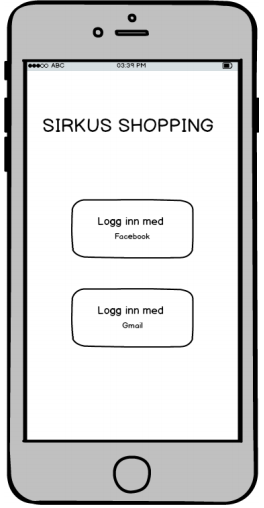
\includegraphics[scale=0.5]{images/prototype1/startskjerm}
\centering %centering the image
\caption{Startskjerm}
\label{fig:startskjerm}
\end{figure}

\noindent I neste trinn får brukeren opp en melding om at dersom hun holder telefonen inntil et produkt kan hun legge det til i handlelisten, vist i Figur \ref{fig:dialogboks}. Ved å trykke “OK” vil boksen lukkes, likt dialogboksene man finner i andre apper.

\begin{figure}[H]
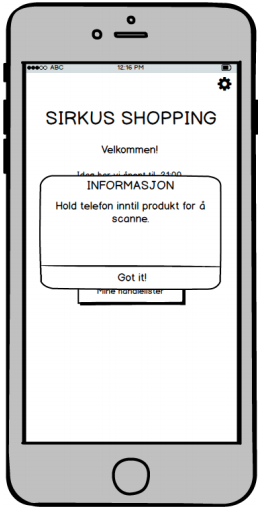
\includegraphics[scale=0.5]{images/prototype1/dialogboks}
\centering %centering the image
\caption{Dialogboks}
\label{fig:dialogboks}
\end{figure}

\noindent For brukere som allerede er logget inn kommer man rett til startsiden. Her ser brukeren logoen til kjøpesenteret, samt informasjon om hvor lenge det holder åpent denne dagen. Brukeren kan velge å lage en ny handleliste, eller å se på eksisterende handlelister. Disse trykkes som knapp. 

\begin{figure}[H]
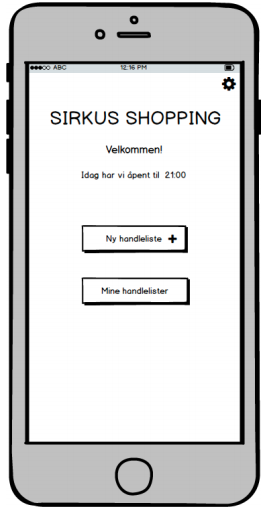
\includegraphics[scale=0.5]{images/prototype1/hjem-skjerm}
\centering %centering the image
\caption{Hjem-skjerm}
\label{fig:hjem-skjerm}
\end{figure}

\noindent Dersom brukeren velger å legge til en ny handleliste må hun skrive inn et navn på handlelisten. Dette gjøres i en dialogboks som kommer opp, og brukeren må bekrefte ved å trykke “OK”. 

\begin{figure}[H]
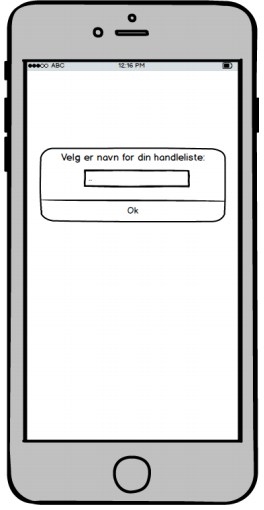
\includegraphics[scale=0.5]{images/prototype1/oppretthandleliste}
\centering %centering the image
\caption{Opprett ny handleliste}
\label{fig:oppretthandleliste}
\end{figure}

\noindent I oversikten “Mine handlelister” kan brukeren se alle handlelistene hun har tilgang til, se Figur \ref{fig:oversikthandlelister} og Figur \ref{fig:oversikthandlelister2}. Det er enten handlelister brukeren har opprettet selv, eller handlelister som andre brukere har delt med vedkommende. På denne siden kan også brukeren legge til flere handlelister ved å trykke på pluss-ikonet. Dette er kjent for brukeren fra andre apper.
\\\\
Nederst på skjermen er det bilde av en søppelbøtte som indikerer at handlelisten kan slettes. Dette gjøres ved å dra handlelisten ned til søppelbøtten. Å bruke søppelbøtte for å slette er et ikon de aller fleste kjenner fra datamaskinen. Å dra elementer til søppelbøtten er også en teknikk man bruker andre steder, som på en datamaskin.

\begin{figure}[H]
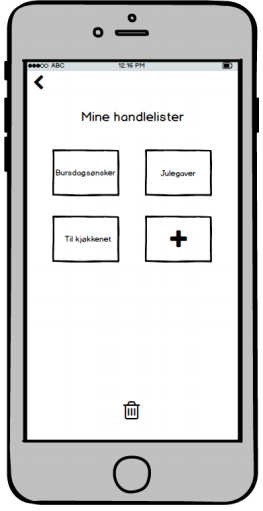
\includegraphics[scale=0.5]{images/prototype1/oversikthandlelister}
\centering %centering the image
\caption{Oversikt over handlelister, variant 1}
\label{fig:oversikthandlelister}
\end{figure}

\begin{figure}[H]
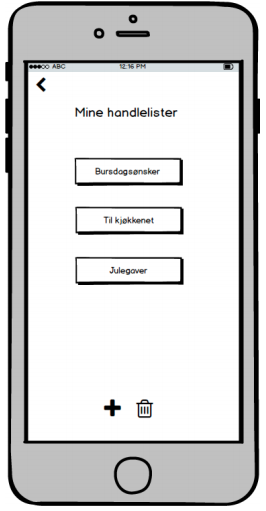
\includegraphics[scale=0.5]{images/prototype1/oversikthandlelister2}
\centering %centering the image
\caption{Oversikt over handlelister, variant 2}
\label{fig:oversikthandlelister2}
\end{figure}

\noindent Når brukeren trykker seg inn på en ønskeliste får vedkommende opp alle varene hun har lagt til i listen. Disse kommer opp med bilde, pris, navn og antall. Det er mulig for brukeren å endre antall av hver vare direkte i listen, eller slette et og et element. Nederst på skjermen kan brukeren se totalsum på varene i listen, og velge å legge alle elementene i listen til i handlekurven.

\begin{figure}[H]
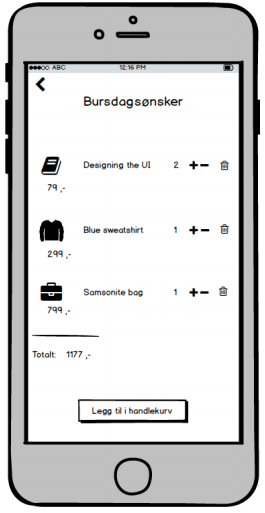
\includegraphics[scale=0.5]{images/prototype1/oversiktliste}
\centering %centering the image
\caption{Oversikt over liste}
\label{fig:oversiktliste}
\end{figure}

Hver vare i handlelisten kan trykkes på for å få opp et mer detaljert skjermbilde av varen. Her er det et stort bilde av varen, pris og størrelse. Varen kan legges til i ønskelisten eller i handlekurven. Dette er det samme skjermbildet som kommer opp når en kunde scanner et produkt med telefonen sin.

\begin{figure}[H]
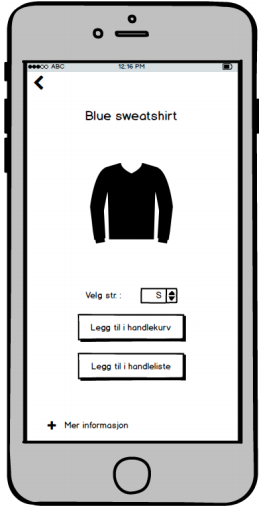
\includegraphics[scale=0.5]{images/prototype1/produkt}
\centering %centering the image
\caption{Visning av produkt}
\label{fig:produkt}
\end{figure}

\noindent Når kunden har fylt opp handlekurven sin med varene hun ønsker kan hun velge å sende ordren. Da vil brukeren få opp et skjermbilde med spørsmål om hun vil betale med Vipps (betalingstjeneste via mobiltelefon) eller om hun vil betale i skranken når hun henter ut varene.

\begin{figure}[H]
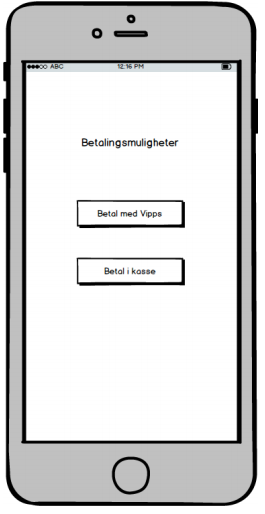
\includegraphics[scale=0.5]{images/prototype1/betalingsmuligheter}
\centering %centering the image
\caption{Betalingsmuligheter}
\label{fig:betalingsmuligheter}
\end{figure}

\noindent Når brukeren har betalt får hun beskjed om hvor lenge det er til hun kan plukke opp varene i varelageret. Dette oppgis i minutter.

\begin{figure}[H]
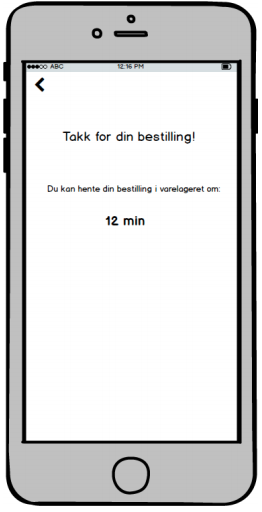
\includegraphics[scale=0.5]{images/prototype1/sluttfortbestilling}
\centering %centering the image
\caption{Sluttført bestilling}
\label{fig:sluttfortbestilling}
\end{figure}

\subsection{Brukertest}
Ved starten av hver test hadde gruppen en sjekkliste som ble gått gjennom før testen startet. Listen var hentet fra forelesningen som omhandlet brukskvalitetstesting\cite{brukskvalitetstesting}. Listen var som følger: 

\begin{enumerate}
    \item Introduser deg selv
    \item Beskriv hensikten med testen
    \item Fortell deltakerne at de kan avbryte når de vil
    \item Beskriv utstyret i rommet og begrensningene til prototypen
    \item Lær bort hvordan man tenker høyt 
    \item Forklar at du ikke kan tilby hjelp under testen
    \item Beskriv oppgaven og introduser produktet
    \item Spør om det er noe de lurer på og kjør testen
    \item Avslutt testen med å la brukeren uttale seg før du samler eventuelle løse tråder
\end{enumerate}

\noindent Mange av disse punktene har den hensikt å gjøre brukeren trygg og komfortabel med testen. Det er viktig å gi brukeren en følelse av kontroll og at han starter testen med en følelse av suksess slik at man får gode og ærlige tilbakemeldinger.
\\\\
Brukeren ble også satt inn i et kort scenario hvor brukeren er på kjøpesenteret for å handle. Siden dette konseptet er ganske annerledes fra en vanlig butikk, ble brukeren satt inn hvordan dette kjøpesenteret fungerte, men gruppen passet på å ikke forklare for mye for at det ikke skulle gå utover testresultatet. Gruppen hadde en genser med en fiktiv strekkode på bordet som testpersonene skulle bruke til oppgavene under testen.

\subsubsection{Testprosedyre}
Papirprototypen ble testet med en test kalt Wizard-of-Oz. Dette er en såkalt low-fidelity prototype-metode\cite[p.~391]{preece}. Den forutsetter at prototypen er basert på software, ettersom brukeren interagerer med softwaren som om han interagerer med produktet. Fordelene med en papirprototype er at den er enkel og billig å lage slik at man kan få tidlig feedback av produktet før man har investert for mye. Siden den er laget av papir og ikke er interaktiv, er det enkelt å forandre designet fort. 
\\\\
Spørsmålene som ble stilt under brukertesten er listet under.

\begin{enumerate}
    \item Du skal lage en oversikt over dine bursdagsønsker. Lista skal hete “bursdagsønsker”.
    \item Du har nå opprettet tre ulike ønskelister. Naviger deg frem til en oversikt over disse.
    \item Legg til en genser i listen over bursdagsønsker. 
    \item Genseren du har lagt i handlelisten er i feil størrelse. Bytt størrelse.
    \item Du vil ikke lenger ha genseren. Fjern genseren.
    \item Du har nå lagt til tre varer til listen og handleturen din er ferdig. Kjøp varene i handlekurven.
    \item Du er på oversikten over dine handlelister. Naviger deg tilbake til startsiden.
    \item Du har fylt opp handlekurven din, men ønsker ikke å kjøpe med én gang. Hva gjør du?
    \item Del genseren med en venn.
\end{enumerate}

\subsubsection{Resultat}
Når man gjennomfører brukertester er det vanlig å gi brukerne et SUS-skjema etter testen. Dette er et skjema for System Usability Scale, og gir brukerne spørsmål om brukervennligheten på en skala fra “sterkt uenig” til “sterkt enig”\cite{usability}. Ut ifra dette kan testerne i ettertid generere en sum som forteller noe om hvor brukervennlig prototypen var. Skalaen går fra 0 til 100, hvor høy sum er best. Alt over 68 regnes som et over gjennomsnittlig resultat.
\\\\
I brukertesten med papirprototypen fikk brukerne i etterkant av testen utdelt et SUS-skjema hvor de svarte på hvor brukervennlig de opplevde prototypen. Resultatene i detalj kan leses i Appendix \ref{App:AppendixB}.
\\\\
Navigasjonsoppgavene og oppretting av lister gikk bra hos alle testdeltakerne. Sletting av genseren var også problemfri. Problemer som gikk igjen hos flere var å forstå forskjellen mellom handlelister og handlekurv, og om de hadde klart å skifte størrelse på genseren fordi det manglet feedback på dette. Det største problemet som alle deltakerne hadde var å få skannet genseren. Man kunne bare ha lagt mobilen inntil genseren så hadde den blitt skannet, men deltakerne letet etter en knapp eller et skjermbilde som viste at appen var klar for skanning. Om deltakerne kom til å skjønne/huske dette ble diskutert i gruppa på forhånd og vi var spente på å se hvordan deltakerne reagerte på dette.

\subsubsection{Analyse}
%-søppelkasseikonet funket
%- la til tab nederst for raskere navigering og for tydeligere skille mellom liste og kurv
%- forandret handleliste til ønskeliste
%- feedback når man skiftet str. Don Norman

Resultatene fra brukbarhetstesten ga gruppen indikasjoner på at noen elementer i prototypen måtte forbedres. Det var ikke alle testpersonene som fikk til oppgavene på tilfredsstillende måte.
\\\\
Når testdeltakerne kom til oppgaven om å legge til en genser i handlekurven, var det mange som ble stille. De skjønte at de skulle skanne strekkoden på genseren, men de ventet på et signal på at det var klart for skanning. Med RFID er mobiltelefonen alltid mottakelig for skanning så man behøver ikke å trykke en plass for å aktivere skanningen, men her hadde designet en mangel på affordance. Det er ingenting som signaliserer at man kan skanne genseren og da tror brukeren at det ikke går ann. 
\\\\
Når man åpnet appen fikk man opp en pop-up som fortalte at man skulle holde telefonen inntil produktet for å skanne. Deltakerne fortalte at de hadde fått med seg denne, men den ble glemt igjen med en gang. Designet her brøt med et av Jacob Nielsens heuristics, recognition rather than recall, som går ut på at brukeren ikke skal behøve å huske informasjon mellom dialoger. Instruksjoner skal være synlige når de trengs\cite[p.~404]{preece}. 
\\\\
Noen av testdeltakerne synes ikke det var helt klart hva forskjellen mellom handlelister og handlekurv var. En grunn til dette var at designet på en handleliste og handlekurven så veldig likt ut, i tillegg til navnene også var veldig like. Poenget med handlelister var at der hadde man varer man ikke skulle kjøpe nå, og at disse listene kunne man dele med andre. Siden man måtte være i butikken for å legge til varer i en liste, passet ikke navnet handleliste. Dette ble derfor forandret til ønskeliste som reflekterte bedre hva som var poenget med listene. 

%norman
%mentale modeller

\subsection{Forbedringer av designet}
%- forandret handleliste til ønskeliste
%- feedback når man skiftet str. Don Norman

Etter å ha gjennomført brukertester bestemte gruppen seg for å utbedre noen ting i designet. Det var flere ting som dukket opp under brukertestene, og gruppen bestemte seg for å endre disse tingene før de gikk videre til neste steg i prosessen.
\\\\
Gruppen fikk tilbakemeldinger om at pop-up vinduet som dukket opp når man logget inn ble trykket “OK” og glemt. Brukerne fikk med andre ord ikke med seg hva som stod i boksen angående scanning av varer. Gruppen valgte derfor å gå bort fra denne løsningen, og gjøre noen endringer på velkomstskjermen. Her ble utseendet og navnet på listene endret, slik at det skulle bli mindre forvirring blant brukerne om hva de ulike elementene var. Ikoner ble lagt til på knappene, slik at brukeren kjenner de igjen senere ved scanning av produkter. 
\\\\
Det ble også lagt til en tab bar nederst på skjermen som hele tiden var synlig, som matchet ikonene på knappene på velkomstskjermen. Dette ble gjort for å forenkle navigeringen i appen siden det var ganske få skjermbilder. Det var å også med på å skille ønskelister fra handlekurv. Når man var på en side, lyste opp det tilhørende ikonet på tab baren for å enklere se hvor man var. 
\\\\
Siden tab baren alltid var synlig ble det mulig å legge til en skann-knapp for brukeren til å trykke på når man skulle skanne en vare. Det var viktig at skann-knappen var synlig hele tiden da brukeren kommer til å skanne varer ofte og man burde slippe å navigere rundt i appen hver gang man skal skanne. 
\\\\
Knappen med “legg til i handlekurv” ble gjort litt større enn knappen med “legg til i ønskeliste” for å få litt mindre fokus på ønskelister siden dette er en valgfri funksjon å bruke. Feltet for “mer informasjon” ble flyttet opp til under bildet av produktet for å vise at det ga informasjon om produktet og ikke om appen. 

%mer her, bilder osv. Bytt ut bildet med et bilde hvor tab baren er med]
\newpage

\section{\textcolor[HTML]{D32F2F}{Designiterasjon 2: Axure}}
\label{design2}

Versjon to av designet ble laget i et program kalt Axure. Dette er et verktøy for prototyping, spesifisering og diagrammer. Her kan man planlegge en prototype, og lage en troverdig app. Det gjør det mulig for gruppen å teste den faktiske opplevelsen av bruk på testpersonene. Modellen blir interaktiv og responderer på klikk. Axure-modellen er med andre ord langt mer avansert enn den forrige prototypen som ble testet med Wizard-of-Oz.

\subsection{Designbeslutninger}
I denne versjonen ble tilbakemeldingene fra brukertesten tatt med. Det ble gjort flere endringer i designet, blant annet ble det lagt inn deleknapp for ønskelister slik at brukeren kan dele direkte på Facebook eller e-post. Boksene i appen ble også endret fra å ha bokser med runde hjørner til å ha firkantede hjørner. Dette ble gjort for å få et pent og gjennomgående design, ikke fordi det hadde noen funksjon ellers i appen. Det siste som ble endret var handlelisten. I dette stadiet er det nødvendig å ta valg innen font, farger og grafiske elementer. Det er veldig viktig med en kosistent design. Dersom alle skjermbildene i applikasjonen følger samme grafiske profil, vil brukeren lettere forstå heltheten, forbedre navigasjonen, samt få et helhetlig inntrykk.

\subsubsection{Navigasjon}
Å ha en meny i produktet ble fort avgjort som nødvendig for en god brukeropplevelse. En meny skal gjerne vise innholdet på en strukturert måte, slik at brukeren skal kunne velge mellom et sett med valg \cite[s.~166]{preece}. Menyer i interface er gjerne plassert i topp- eller bunnlinjen av skjermen, eller langs venstre side. Det er mange måter å gjøre dette på, og eksempler er lister, drop-down, pop-up, kontekstuelle, ekspanderende og scrolling. Gruppen valgte å gå for en enkel meny, siden det er få sider i designet og målet var at appen skulle være enklest mulig. Ved å bruke denne menyen blir det enklere for brukeren å navigere seg mellom de forskjellige skjermbildene. 

\subsubsection{Farger}
Farger er også viktig for å få en ideell brukeropplevelse. Farger i seg selv signaliserer mye til brukeren, men også valg av farger å komponere er avgjørende. Å lese en grønn tekst på rød bakgrunn er slitsomt for øynene, og det samme er turkis på grå bakgrunn\cite{esthetics}. Det optimale er svart på hvitt for god lesbarhet, men det velges ofte farger for å sprite opp designet. Da er det vanlig å lage en fargepalett, hvor de samme fargene går gjennom i hele designet. Siden Sirkus shopping har en rød profil, valgte gruppen å bruke denne rødfargen som primærfarge. Videre utformet gruppen en fargepalett på \textcolor[HTML]{0000FF}{\underline{www.materialpalette.com}}, som vist i Figur \ref{fig:fargepalett}.

\begin{figure}[H]
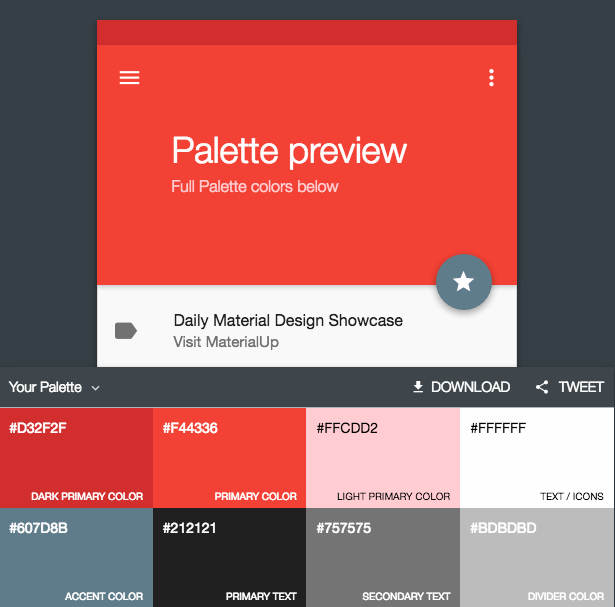
\includegraphics[scale=0.65]{images/colors.png}
\centering %centering the image
\caption{Applikasjonens fargepalett}
\label{fig:fargepalett}
\end{figure}

\subsubsection{Fonter}
Gruppen valgte å bruke Raleway som er en estetisk ren og lettleselig font. Det er viktig å ha en kontinuitet på fontstørrelse, og at hver størrelse har en mening. Det vil si å ha en fast stor størrelse på overskrifter, en mindre font på tekst for knapper, og en mindre font for infotekst. Med tanke på at applikasjonen skal benyttes av voksne mennesker, er det viktig å ha stor nok font for bra lesbarhet.

\subsubsection{Skjermbilder}
I Figur \ref{fig:interaksjon1} og Figur \ref{fig:interaksjon2} er det vist et diagram for å vise hvordan de forskjellige skjermbildene samhandler med hverandre. Figur \ref{fig:interaksjon1} viser hvordan du går fra login-skjerm til hovedmenyen. Herfra har du tre valg, der du kan enten opprette en ny ønskeliste, få en oversikt over ønskelistene dine, eller gå direkte til handlekurv. 

\begin{figure}[H]
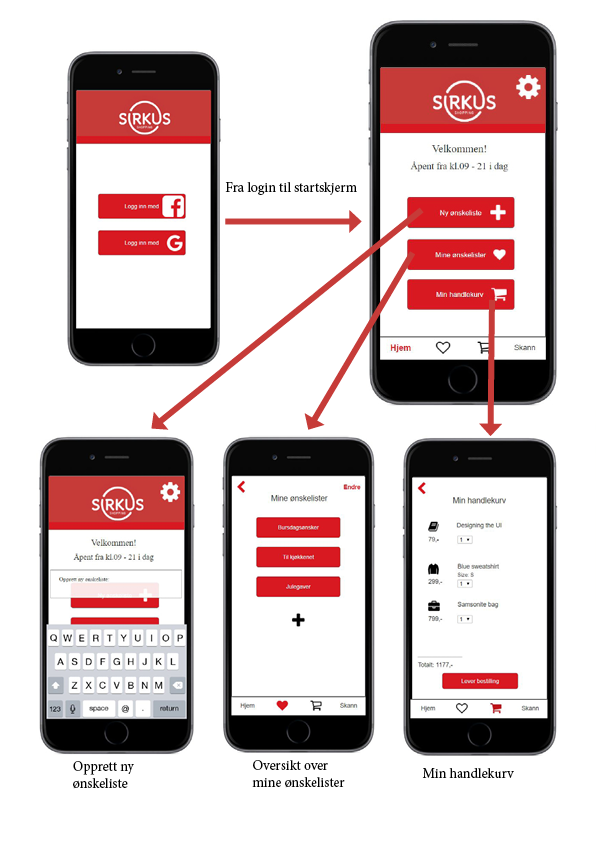
\includegraphics[scale=0.70]{images/axurebilder/axure-interaksjon.png}
\centering %centering the image
\caption{Interaksjon del 1}
\label{fig:interaksjon1}
\end{figure}

\noindent Figur \ref{fig:interaksjon2} viser hvordan brukeren kan trykke seg inn på et ønsket produkt fra handlekurven og deretter endre f.eks. størrelse. Dersom brukeren trykker på "Lever bestilling" blir hun dirigert til en ny skjerm som gir mulighet til å velge betalingsløsning. Herfra velger hun enten Vipps eller tradisjonell betaling i kasse. Etter å ha valgt her får brukeren et nytt skjermbilde som viser hvor lenge det er til hun kan hente varene sine. Det siste eksemplet viser hvordan man kan dele en ønskeliste via forskjellige sosiale plattformer.

\begin{figure}[H]
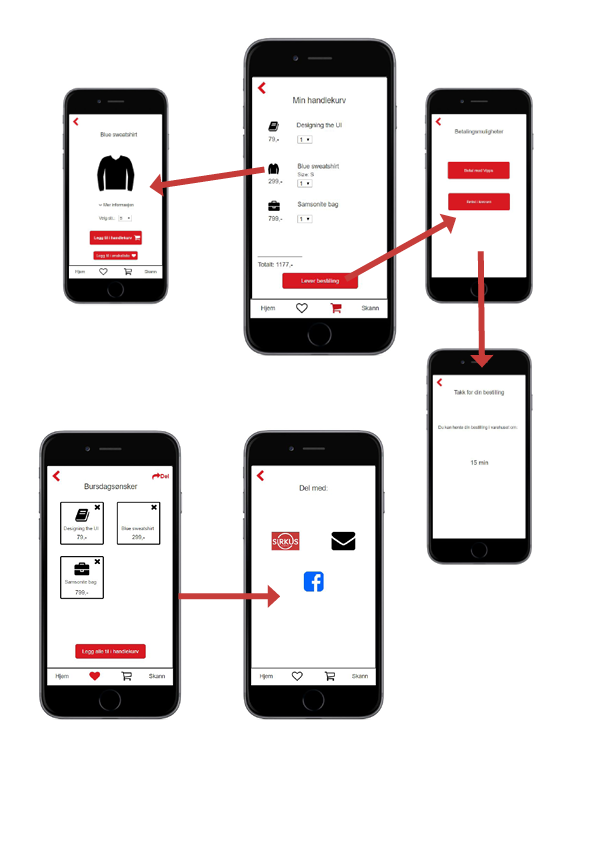
\includegraphics[scale=0.75]{images/axurebilder/interaksjon2}
\centering %centering the image
\caption{Interaksjon del 2}
\label{fig:interaksjon2}
\end{figure}

%flytdiagram

\subsection{Brukertest}
Da det skulle brukertestes gang nummer to, var det blitt laget en prototype med Axure. Denne prototypen lignet mye på det gruppen så for seg som det ferdige produktet, og denne brukertesten ble da av typen high-fidelity. Det vil si at den ligner mye på det ferdige produktet, og har flere funksjonaliteter enn en low-fidelity-prototype \cite[s.~391]{preece}. Å teste med high-fidelity har mange fordeler, siden det gir brukeren en nær opplevelse av hvordan det ferdige produktet vil se ut, men har også store kostnader. Det krever langt mer tid å utvikle en Axure-prototype enn en prototype i papir, slik gruppen brukte i Wizard-of-Oz-testen.

\subsubsection{Testprosedyre}
Den første brukertesten av Axure-prototypen ble gjort på lab hvor det ble brukt eyetracking. Dette er et kamera som er festet på undersiden av skjermen som detekterer hvor øynene ser. Før testen starter kalibrerer man programmet mot øynene, slik at man er sikker på at punktene brukeren ser på blir registrert. Deretter setter man kameraet på opptak, og vil da kunne se hvor brukeren ser til enhver tid, samt hvordan øynene forflytter seg over skjermen.
%les på forelesningsslide om eyetracking
\\\\\
Testspørsmålene som ble brukt under brukertesten var relativt like de som ble stilt i den forrige brukertesten. Dette ble gjort med hensikt, fordi det da er lettere å sammenligne resultatene. Noen endringer måtte likevel gjøres, siden appen hadde fått noen endrede funksjoner. Testspørsmålene er listet under.

\begin{enumerate}
    \item Logg inn med valgfritt innloggingsverktøy
    \item Du skal lage en oversikt over dine bursdagsønsker. Lista skal hete “bursdagsønsker”.
    \item Legg til en genser i listen over bursdagsønsker.
    \item Naviger deg tilbake til oversikten over mine ønskelister.
    \item Du er på oversikten over dine ønskelister. Naviger deg tilbake til startsiden.
    \item Genseren du har lagt i ønskelisten er i feil størrelse. Bytt størrelse.
    \item Del listen “Bursdagsønsker” med en venn. Velg selv delingsplattform.
    \item Slett ønskelisten “Julegaver”
    \item Gjennomfør et kjøp av denne genseren.
\end{enumerate}

\subsubsection{Resultat}
Den første oppgaven som ble gitt var å logge inn med et valgfritt innloggingsverktøy. Her valgte testpersonen å logge inn med Facebook, med en kommentar om at hun egentlig var litt skeptisk til å logge inn via dette. Ellers ble oppgaven løst uten problem. 
I oppgave to ble testpersonen bedt om å lage en oversikt over sine bursdagsønsker, og listen skulle hete “bursdagsønsker”. Brukeren trykket på ikonet for ny ønskeliste, skrev inn navn på listen og trykket “return” på tastaturet. Oppgaven ble løst vellykket.
\\\\
Neste oppgave var å legge til en genser i listen over bursdagsønsker. Her måtte brukeren tenke seg om før hun fant riktig løsning. Hun vurderte å trykke “legg til handlekurv” men konkluderte med at det ikke var det hun skulle gjøre. Hun trykket seg heller tilbake, og lette etter hvor det skulle gjøres. Siden det ikke ble gitt god nok informasjon i forkant av testen måtte testlederen bryte inn og minne om at produkter kan legges til ved å scanne varen. Da denne informasjonen ble påpekt hadde brukeren ingen problemer med å legge til varen i ønskelisten.
\\\\
Oppgaven var deretter å navigere seg tilbake til oversikten over ønskelister. Dette ble løst uten problem. Herfra fikk testpersonen i oppgave å navigere seg til startsiden. Hun nevner at hun både kan trykke på pil tilbake, og på huset nede i hjørnet for å komme seg tilbake. Hun velger å trykke på pilen. Oppgaven er løst.
\\\\
Neste oppgave testpersonen ble gitt var å endre størrelsen på genseren hun la til i ønskelisten. Brukeren lurer på hvilken størrelse hun skal endre til, men bestemmer seg for å bytte fra XS til M. Oppgaven er løst. Brukeren blir så bedt om å dele ønskelisten med en venn på en egenvalgt delingsplattform. Brukeren trykker på pilen i høyre hjørne og deler via Facebook. Hun får ingen respons på valget sitt, men blir fortalt at hun nå har delt listen. Deretter får hun oppgave i å slette ønskelisten kalt “Julegaver”. Brukeren går tilbake til oversikten over lister, og finner julegavelisten. Hun trykker på endre og sletter listen. Oppgaven er utført. Til slutt blir testpersonen bedt om å gjennomføre et kjøp av genseren. Hun legger genseren i handlekurven, leverer bestilling, betaler med Vipps og får beskjed om at varen kan hentes om 15 minutter.
\\\\
Etter testen tok testleder en prat med testpersonen om opplevelsen. Hun sa at noen ganger visste hun ikke hva hun skulle gjøre, men det gikk stort sett greit. Briefingen i forkant av testen ble ikke gjort godt nok, så testpersonen fikk ikke med seg det faktum at hun oppholdt seg på senteret. Ut over det mente hun at det nesten var umulig å gjøre feil i appen, siden det stort sett var to valg å velge mellom hele veien. Testlederen spurte om hva testpersonen tenkte om bruk av symboler som hjerte og handlevogn. Brukeren tok ikke i bruk menylinjen, med argument om at de var like på listene og i menyen. Hun kunne brukt de, men savnet tekst under ikonene i menyen. Hun skjønte at hjerte betydde favoritt, siden hjerte eller stjerne ofte symboliserer dette, men tok dem likevel ikke i bruk. Hadde hun brukt appen flere ganger hadde hun nok brukt ikonene, i følge henne selv. Konklusjonen fra testpersonen var at appen var enkel og ikke hadde unødvendige funksjoner. En siste kommentar var at det kanskje var unødvendig med ønskelisteikoner på forsiden.

\subsubsection{Analyse}
Gruppen valgte å bruke punkter og ikke ''heatmap'' for eyetrackingen, da skjermen er ganske liten og man mest sannsynlig kom til å se på midten av skjermen mye mer enn resten av skjermen. Med punkter får man se når og hvor man flytter blikket hele tiden.
\\\\
Siden det er ganske få elementer per skjermbilde og det meste i appen er sentrert, søker testpersonen som oftest i et vertikalt mønster opp og ned. Man kan observere at testpersonen skanner fort over elementene og bruker lite tid på å se nøye etter. Dette er ikke et problem her siden de fleste ordene og elementene er små at testpersonen får de med seg uten å måtte lese de. 
\\\\
Figur \ref{fig:eyetrack1} viser et bilde som er tatt noen sekunder etter at testpersonen har åpnet appen og startet med første oppgave. Her kan man se at testpersonen starter øverst med å lese åpningstidene og se på logoen. Etterhvert skanner hun nedover hovedmenyen for å se hva hun skal gjøre for å løse første oppgave. Hun ser ikke på menylinjen i det hele tatt før hun trykker på \textit{Ny ønskeliste} og fortsetter oppgaven. Det er en observasjon som gjentar seg gjennom hele testen. Blikket går veldig sjeldent ned på menylinjen, som bekrefter det testpersonen uttalte om at menylinjen fikk lite fokus siden man kunne navigere seg ved bruk av hjemskjermen og tilbakeknapper. 

\begin{figure}[H]
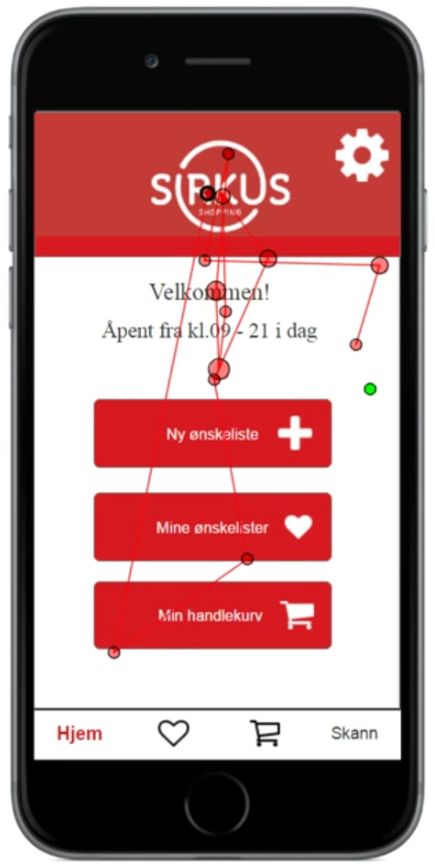
\includegraphics[scale=0.5]{images/eyetracking/eyetrack1.png}
\centering %centering the image
\caption{Eyetracking}
\label{fig:eyetrack1}
\end{figure}

%Videoen som ble tatt opp under testen
\noindent Det må nevnes at å brukerteste en applikasjon for mobiltelefon på en datamaskin ikke er helt ideelt. På en smarttelefon bruker man knapper på telefonen og touch-skjerm for å navigere i appen. På en datamaskin brukes en mus, så resultatene er ikke helt korrekt. 

\newpage

\section{\textcolor[HTML]{D32F2F}{Videre utvikling}}
\newpage

\section{\textcolor[HTML]{D32F2F}{Oppsummering}}
Det viktigste vi lærte i prosjektet var hvor nyttig det var med brukertester.
brukere tenker annerledes enn de som lager
vite hvilke behov som finnes
tenke høyt under test
%Gruppen har samarbeidet godt gjennom prosessen, og


\subsection{Refleksjon om tverrfaglige grupper}
I gruppen som ble satt sammen var alle medlemmene informatikkstudenter. Gruppen ble dermed ikke like tverrfaglig som mange av de andre gruppene i emnet, men det fungerte stort sett greit. Det kunne selvfølgelig vært en fordel å for eksempel ha en student fra produktdesign når det skulle lages og printes poster, men gruppen løste oppgaven godt selv uten ressursene som mange andre grupper hadde.

\subsection{Retrospekt}
Dersom vi skulle gjort prosjektet en gang til er det noen ting vi ville gjort annerledes. For det første ville vi ha kjørt flere observasjoner, og vi burde ikke ha spisset inn så tidlig som vi gjorde.

\subsection{Videre arbeid med produkt}
Prototypen vi har kommet fram til skiller seg klart fra andre apper som finnes på markedet i dag, og vil gi brukerne en helt ny måte å handle på. Vi mener at dette absolutt kan være verdt å satse på. Det forutsetter at man får med seg handlesentrene på ideen, men vi tror at dette kan hjelpe mange kunder med å handle mer effektivt. På denne måten kan man sammenligne priser og produkter, og det blir også mulig for kunden å se antall på lager. Dette er noe mange brukere nevnte i spørreundersøkelsen vi gjorde, og det tyder på at dette er noe forbrukerne savner. Løsningen vi har laget vil også gjøre det raskt og lettvint for forbrukere på storhandel å handle. De trenger ikke bære på mange handleposer, eller gå rundt med stor handlevogn. Alle varene hentes til slutt, ferdig pakket, og kan bæres rett inn i bilen.
\\\\
Om butikkene vil se på dette som en god løsning er ikke sikkert, men vi tror at dersom man får kartlagt alle behov og finner en god løsning av alle aspekt vil dette kunne trekke mange kunder. Ved å ha en totalpris i bunn av handlelisten blir kunden observant på hva det koster, og det kan gjøre at kunden handler for mindre beløp. Det er det ikke sikkert butikkene liker. Det blir også langt vanskeligere med mersalg når brukeren ikke betaler i kassen i hver butikk, men kun til slutt for hele handleopplevelsen.
\\\\
Løsningen vi har kommet opp med krever en annen disponering av ressurser enn man ser i handlesentrene i dag. Med vår løsning vil man ikke trenge personell i kassen, men heller ute i butikken som kan hjelpe kundene. Det vil da være ved å finne riktig størrelse, besvare spørsmål om produktet og gi råd til hva man burde velge. 


\newpage

\section{\textcolor[HTML]{D32F2F}{Kilder}}
\begin{thebibliography}{30}
%husk alfabetisk!
\bibitem{kahn}
Kahn, R. and Cannell, C. (1957) \textit{The Dynamics of Interviewing}. John Wiley \& Sons Inc., New York.

\bibitem{preece}
Preece, Jennifer; Sharp, Helen; Rogers, Yvonne. (2015) \textit{Interaction Design – Beyond human-computer interaction}. 4th edition. UK: Wiley.

\bibitem{sirkus}
Sirkus Shopping. (u.å.) \textit{Butikker}. [Internett] Trondheim: Sirkus Shopping. Tilgjengelig fra: \\\texttt{http://sirkusshopping.no/} [Lest 14. november 2016]

\bibitem{brukersentrert}
Svanæs, Dag. (2016) \textit{Brukersentrert design}. Forelesningsslide, IT3402, NTNU. Tilgjengelig på It’sLearning. [Lest 18. oktober 2016]

\bibitem{feltstudie}
Svanæs, Dag. (2016) \textit{Feltstudie og poster}. Forelesningsslide, IT3402, NTNU. Tilgjengelig på It’sLearning. [Lest 15. oktober 2016]

\bibitem{prosjektoppgaven}
Svanæs, Dag. (2016) \textit{Prosjektoppgaven: Shoppingsentre}. Forelesningsslide, IT3402/TPD4134, NTNU. Tilgjengelig på It’sLearning. [Lest 18. oktober 2016]

\bibitem{servicedesign}
Svanæs, Dag. (2016) \textit{Forelesning service design}. Forelesningsslide, IT3402, NTNU. Tilgjengelig på It’sLearning. [Lest 21. november 2016]

\bibitem{usability}
Usability.gov. (u.å.) \textit{System Usability Scale (SUS)} [Internett] Washington: U. S. Department of Health \& Human Services. Tilgjengelig fra:\\ \texttt{https://www.usability.gov/how-to-and-tools/methods/system-usability-scale.html} [Lest 14. november 2016]

\bibitem{brukskvalitetstesting}
Øritsland, Trond Are. (2016) \textit{Brukskvalitetstesting}. Forelesningsslide, TPD4134, NTNU. Tilgjengelig på It’sLearning. [Lest 18. november 2016]

\bibitem{esthetics}
Øritsland, Trond Are. (2016) \textit{Esthetics}. Forelesningsslide, TPD4134, NTNU. Tilgjengelig på It’sLearning. [Lest 18. november 2016]

\bibitem{paperprototype}
Øritsland, Trond Are. (2016) \textit{Paper prototype}. Forelesningsslide, TPD4134, NTNU. Tilgjengelig på It’sLearning. [Lest 15. oktober 2016]

\bibitem{guidelines}
Øritsland, Trond Are. (2016) \textit{User Interface Guidelines}. Forelesningsslide, IT3402, NTNU. Tilgjengelig på It’sLearning. [Lest 15. oktober 2016]

\end{thebibliography}
\newpage

\begin{center}
\vspace*{5.5cm}
\huge{\textbf{\textcolor[HTML]{D32F2F}{Appendix}}}
\end{center}
\newpage 

\appendix
\section{\textcolor[HTML]{D32F2F}{Spørreundersøkelse – Resultater}} \label{App:AppendixA}

Gruppen fikk inn 51 svar på spørreundersøkelsen som ble sendt ut i forbindelse med prosjektet. Resultatene følger.

\begin{figure}[H]
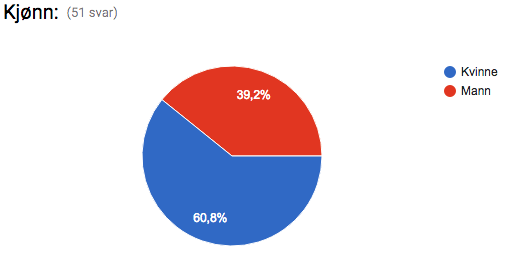
\includegraphics[scale=0.6]{images/sporreundersokelse/kjonn}
\centering %centering the image
\caption{Kjønn}
\label{fig:kjonn}
\end{figure}

\begin{figure}[H]
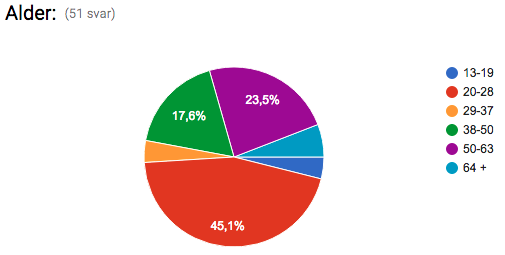
\includegraphics[scale=0.6]{images/sporreundersokelse/alder}
\centering %centering the image
\caption{Alder}
\label{fig:alder}
\end{figure}

\begin{figure}[H]
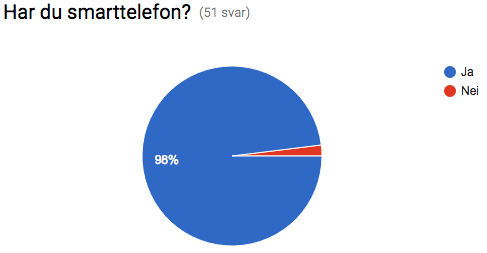
\includegraphics[scale=0.6]{images/sporreundersokelse/smarttelefon}
\centering %centering the image
\caption{Eier smarttelefon}
\label{fig:smarttelefon}
\end{figure}

\begin{figure}[H]
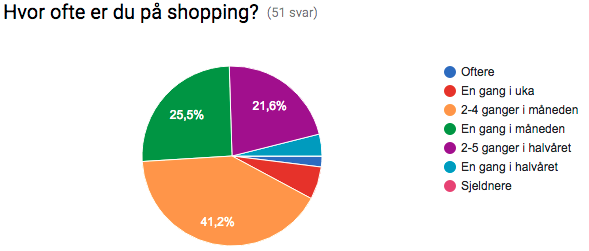
\includegraphics[scale=0.6]{images/sporreundersokelse/shopping}
\centering %centering the image
\caption{Shoppingfrekvens}
\label{fig:shopping}
\end{figure}

\begin{figure}[H]
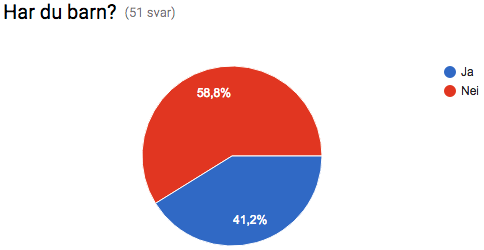
\includegraphics[scale=0.6]{images/sporreundersokelse/barn}
\centering %centering the image
\caption{Barn}
\label{fig:barn}
\end{figure}

\begin{figure}[H]
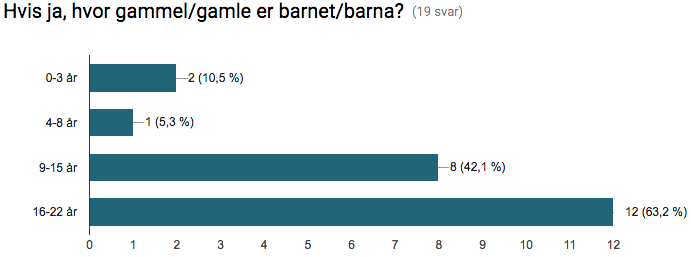
\includegraphics[scale=0.6]{images/sporreundersokelse/alderbarn}
\centering %centering the image
\caption{Alder på barn}
\label{fig:alderbarn}
\end{figure}

\noindent \large{\textbf{Hvis ja, hvordan opplever du handleturen med barna?}}
\begin{itemize}
    \item Trivelig
    \item Trivelig
    \item Stressende
    \item OK
    \item Hyggelig. Får gode råd og tips av nesten voksen datter.
    \item Tragisk, de ber alltid om noe
    \item Helt OK
    \item Bra
    \item Litt stressende :)
    \item Barna er voksne…
    \item Koselig
    \item Er så voksne at det bare er hyggelig
    \item Hyggelig, får råd og hjelp
\end{itemize}

\begin{figure}[H]
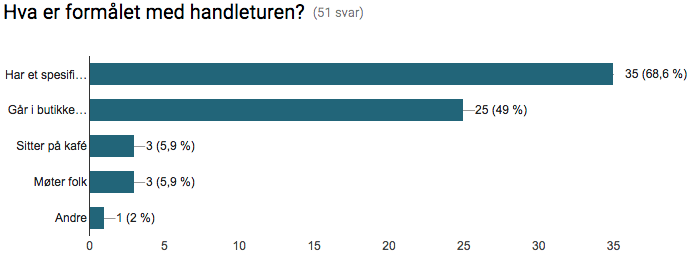
\includegraphics[scale=0.6]{images/sporreundersokelse/formal}
\centering %centering the image
\caption{Formål med handletur}
\label{fig:formal}
\end{figure}

\begin{figure}[H]
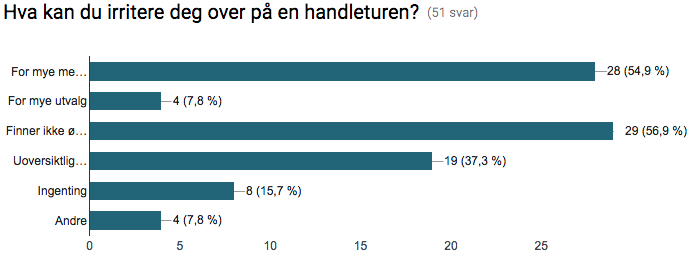
\includegraphics[scale=0.6]{images/sporreundersokelse/irritasjonsmoment}
\centering %centering the image
\caption{Irritasjonsmoment}
\label{fig:irritasjonsmoment}
\end{figure}

\begin{figure}[H]
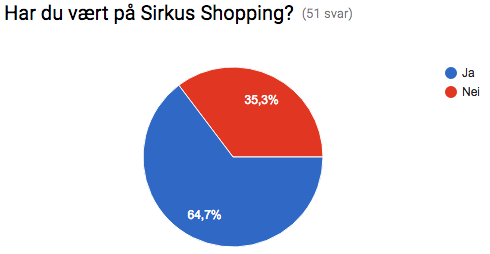
\includegraphics[scale=0.6]{images/sporreundersokelse/besokt}
\centering %centering the image
\caption{Besøkt Sirkus shopping}
\label{fig:besokt}
\end{figure}

\noindent \large{\textbf{Hvis ja, hvordan opplever du handleturen på Sirkus shopping?}}
\begin{itemize}
    \item Ok
    \item Ok
    \item Bra
    \item Bra
    \item Helt OK
    \item Helt ok
    \item Rotete
    \item Rotete
    \item Fint
    \item Fint
    \item Hva er Sirkus Shopping?
    \item Veldig bra
    \item Fin
    \item Rolig affære, finner sjelden noe
    \item Husker ikke
    \item Rolig
    \item Veldig fint kjøpesenter, lett å finne fram
    \item Bra!
    \item Litt rar planløsning, men var ikke et så masete sted
    \item Stort senter, vanskelig å få god oversikt. Behagelig pga mindre folk.
    \item Liker sirkus. Åpent og god oversikt, pleier ikke være så mye folk
    \item OK
    \item Litt uoversiktlig
    \item Den var bra! et lett og finne fram og ryddig
    \item Bra
    \item Tilfredsstillende
    \item Veldig stort og uoversiktlig
    \item God opplevelse, nyttige sofaer dårlig for menn, utvalg
    \item Helt greit. God plass, enkel parkering, kan få vasket bilen mens du handler, litt “andre” butikker
    \item Husker ikke. Lenge siden jeg var der
    \item Helt greit. Grei parkering, får vasket bilen mens du handler. Litt annerledes butikker.
\end{itemize}

\noindent \large{\textbf{Har du brukt apper for å forbedre shoppingen tidligere, evt. hvilke?}}
\begin{itemize}
    \item Nei
    \item Ja, mattilbud
    \item Nei, teknologi er ikke noe for meg
    \item Ingen
    \item Prisjakt.no, finn, google-søk om varene
    \item ikke en app laget for kjøpesenter, men bestilt varer på app tidligere og fått de levert på døra
    \item Zalando
\end{itemize}

\begin{figure}[H]
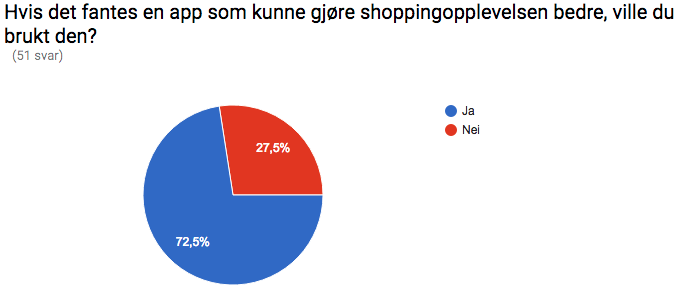
\includegraphics[scale=0.6]{images/sporreundersokelse/brukeapp}
\centering %centering the image
\caption{Vil bruke app}
\label{fig:brukeapp}
\end{figure}

\noindent \large{\textbf{Hvis nei, hvorfor?}}
\begin{itemize}
    \item For mange apper
    \item For mange apper
    \item Fordi jeg vil ikke i butikken i det hele tatt
    \item Shopper lite
    \item Hva er en app?
    \item Bestiller alt online
    \item Jeg shopper så og si aldri
    \item Synes det er lite vits, da jeg uansett er på shopping for å titte og se meg rundt
    \item Jeg kan bruke den hvis det er noe spesifikt jeg trenger som jeg vil se etter på tilbud. Ellers så liker jeg å gå rundt i butikker og prøve ulike varianter av et produkt før jeg gjør et kjøp
    \item Er ikke så ofte på shopping at jeg føler jeg har behov for en shoppingapp. Tar bare plass på telefonen. Men kommer selvfølgelig an på hva en slik app inneholder også.
    \item Enda mer å styre med bare
    \item Ser ikke behovet
    \item Ikke interessert
\end{itemize}

\noindent \large{\textbf{Har du forslag til funksjoner en shopping-app kan inneholde??}}
\begin{itemize}
    \item Nei
    \item Lagerbeholdning, pris, tester
    \item Viser hva er i butikken - størrelser utvalg osv. for å unngå bomturer
    \item Litt usikker
    \item Oversikt over butikker
    \item Hvor man finner nærmeste toalett, at man kan legge inn at man f.eks.. ønsker å kjøpe hvit skjerf så kommer forslag til butikker som har dette skjerfet
    \item Oversikt over nåværende tilbud
    \item nei dessverre
    \item Rabatt koder
    \item Alle butikker, priser og salg hos hver enkelt kjøpesenter
    \item Prissammenligning
    \item Lageroversikt
    \item Tilbud fra butikkene
    \item Salstilbud, oversikt over butikker
    \item Oversikt over hva som faktisk finnes i de ulike butikkene, ikke bare online
    \item Oversikt over hvor jeg kan finne ønsket produkt
    \item Rabattkort/kuponger?
    \item App er ut, Finn på noe nytt
    \item rabatter, kart over senter, en knapp som får små barn til å slutte å gråte
    \item Oversikt over rabatter og tilbud, info om hvor crowded en butikk er (så jeg kan unngå butikken), hvem som er på jobb i butikken jeg vil besøke (hvis det er spesielle selgere man har opparbeidet seg relasjon med)
    \item Konkurranser og ekstra tilbud forbeholdt brukere av appen (da ville jeg ha lastet den ned, selv om jeg ikke er på shopping så ofte). Kart med oversikt over de ulike butikkene kan også være nyttig.
    \item Oversikt over tilgjengelige produkter og pris
    \item Strekkodescanner som gir deg nyttig info om produktet, prissammenligning, peer reviews og promovideo
    \item Størrelser på klær sko. Nyheter.
    \item Kart over shoppingsenteret med gps som finner din posisjon. Kan også ha et side med alle tilbud på senteret.
    \item Oversikt over produkter, størrelser, hvor man finner de, pris, antall og om de evt. er på lageret om de ikke er ute i butikken. Når produktet evt kommer inn igjen om det ikke finnes p.t.
    \item Kupp
    \item Babes of the day
    \item ukestilbud/dagstilbud. hvilke butikker som er tilgjengelig og hvor de holder til/åpningstider. hvor man kan kjøpe mat og kanskje en slags for kunde-rating for andre brukere på appen så man kan ta utgangspunkt i det når man skal ha “matpause” fra shoppingen. en kommentarfelt til hver butikk hvor man kan legge en tilbakemelding etter endt shopping, og slik at andre potensielle kunder kan se om servicen er bra der osv.
    \item Nei
    \item Bilde av klærne på en som er ca samme strl
    \item Nærmeste utsalg av produktet
    \item Salgsvarer. Sesongvarer
    \item vet ikke
    \item Merker, hvilke butikker har hvilke merker
    \item Kart over kjøpesenter for å finne butikkene. Søke etter hvilken butikk som har den varen man ønsker å kjøpe
    \item Hvilke butikker som har hvilke merker
\end{itemize}

\newpage
\section{\textcolor[HTML]{D32F2F}{Observasjonsskjema for test 1}} \label{App:AppendixB}

\begin{table}[H]
    \caption{Sivilingeniør 58 år, dame}
    \label{tab:observasjon1_1}
    \centering
    \begin{tabular}{L{15em}  L{15em} L{15em}}
        \rowcolor[HTML]{D32F2F}
        \textbf{\textcolor{white}{Task}} & \textbf{\textcolor{white}{Obeservation during execution}} & \textbf{\textcolor{white}{Conversation and discussion}}\\
        \rowcolor[HTML]{E6E6E6}
        1. Du skal lage en oversikt over dine bursdagsønsker. Lista skal hete “bursdagsønsker”. & “Bra å få vite åpningstid”. Laget lista. Bra & \\
        2. Du har nå opprettet tre ulike handlelister. Naviger deg frem til en oversikt over disse. & Trykket på Mine handlelister. Bra &  \\
        \rowcolor[HTML]{E6E6E6}
        3. Legg til en genser i listen over bursdagsønsker. & Går på bursdagsønsker. Trykker på legg til i handlekurv. Tenker lenge. Kommer etterhvert på at man kan scanne klær. Velger størrelse. Legg i handlekurv & Glemmer beskjeden i begynnelsen. Savner et skjermbilde som gjør klar for scanning.\\ 
        4. Genseren du har lagt i handlelisten er i feil størrelse. Bytt størrelse. & Trykker tilbake. (Kommer da til bilde av genseren. Vet ikke om det er det som skal skje) Skifter størrelse. Trykker legg i handlekurv. & Ønsker en beskjed om hva som har skjedd.\\
        \rowcolor[HTML]{E6E6E6}
        5. Du vil ikke lenger ha genseren. Fjern genseren. & Trykker på søppelbøtta. Bra & \\
        6. Du har nå lagt til tre varer til listen og handleturen din er ferdig. Kjøp varene i handlekurven. & Trykker lagre. Går inn på bursdagsønsker igjen. “Har jo lagt det i handlekurva før?” Trykker legg til i handlekurv. Lever bestilling. Betal i kasse. & Ville ikke ha brukt systemet hvis man må vente til slutt. Kan like godt ta med varene selv.\\
        \rowcolor[HTML]{E6E6E6}
        7. Du er på oversikten over dine handlelister. Naviger deg tilbake til startsiden. & Trykker tilbake & \\
        8. Du har fylt opp handlekurven din, men ønsker ikke å kjøpe med én gang. Hva gjør du? & Trykker lagre & \\
    \end{tabular}
\end{table}

\noindent SUS result: 57,5

\begin{table}[H]
    \caption{Student 24 år, jente}
    \label{tab:observasjon1_2}
    \centering
    \begin{tabular}{L{15em}  L{15em} L{15em}}
        \rowcolor[HTML]{D32F2F}
        \textbf{\textcolor{white}{Task}} & \textbf{\textcolor{white}{Obeservation during execution}} & \textbf{\textcolor{white}{Conversation and discussion}}\\
        \rowcolor[HTML]{E6E6E6}
        1. Du skal lage en oversikt over dine bursdagsønsker. Lista skal hete “bursdagsønsker”. & Bra. & \\
        2. Du har nå opprettet tre ulike handlelister. Naviger deg frem til en oversikt over disse. & Trykker tilbake. Mine handlelister. Bra &  \\
        \rowcolor[HTML]{E6E6E6}
        3. Legg til en genser i listen over bursdagsønsker. & Går på bursdagsønsker. Trykker legg til i handlekurv. Går tilbake til hovedmeny. Bursdagsønsker. Legg til i handlekurv. Leter etter en plass for å scanne. Gir henne et hint. Scanner genseren. Trykker legg til i handleliste. & Husker ikke at man bare skal scanne. Kunne hatt en knapp i hjørnet.\\
        4. Genseren du har lagt i handlelisten er i feil størrelse. Bytt størrelse. & Sletter genseren. Scanner den på nytt og legger til en ny. & \\
        \rowcolor[HTML]{E6E6E6}
        5. Du vil ikke lenger ha genseren. Fjern genseren. & Trykker søppelbøtta & \\
        6. Du har nå lagt til tre varer til listen og handleturen din er ferdig. Kjøp varene i handlekurven. & Trykker legg i handlekurv og lever bestilling. Gikk bra. & \\
        \rowcolor[HTML]{E6E6E6}
        7. Du er på oversikten over dine handlelister. Naviger deg tilbake til startsiden. & Ok & \\
        8. Du har fylt opp handlekurven din, men ønsker ikke å kjøpe med én gang. Hva gjør du? & Går til bursdagsønsker. (Gir henne handlekurvbilde, mangler noe i mellom her). Trykker lagre. & Skjønner ikke helt forskjell på liste og kurv. Hvis du scanner og skal kjøpe, legger du i kurv. Hvis du ikke skal kjøpe den, er det noe du ønsker deg.\\
    \end{tabular}
\end{table}

\noindent SUS result: 87,5

\begin{table}[H]
    \caption{Student 22 år, gutt}
    \label{tab:observasjon1_3}
    \centering
    \begin{tabular}{L{15em}  L{15em} L{15em}}
        \rowcolor[HTML]{D32F2F}
        \textbf{\textcolor{white}{Task}} & \textbf{\textcolor{white}{Obeservation during execution}} & \textbf{\textcolor{white}{Conversation and discussion}}\\
        \rowcolor[HTML]{E6E6E6}
        1. Du skal lage en oversikt over dine bursdagsønsker. Lista skal hete “bursdagsønsker”. & Bra. & \\
        2. Du har nå opprettet tre ulike handlelister. Naviger deg frem til en oversikt over disse. & Trykker tilbake. Bra &  \\
        \rowcolor[HTML]{E6E6E6}
        3. Legg til en genser i listen over bursdagsønsker. & Trykker bursdagsønsker. Scanner med en gang. Velger størrelse. Trykker legg til i handleliste. Bra & \\
        4. Genseren du har lagt i handlelisten er i feil størrelse. Bytt størrelse. & Trykker på genseren som ligger i lista. Bytter størrelse. Trykker tilbake. Skjønte ikke helt hva han gjorde. “Er størrelsen endret nå?” & \\
        \rowcolor[HTML]{E6E6E6}
        5. Du vil ikke lenger ha genseren. Fjern genseren. & Trykker på søppelbøtta. Bra & \\
        6. Du har nå lagt til tre varer til listen og handleturen din er ferdig. Kjøp varene i handlekurven. & Trykker legg til i handlekurv. Lever bestilling. Betal med vipps. Bra & \\
        \rowcolor[HTML]{E6E6E6}
        7. Du er på oversikten over dine handlelister. Naviger deg tilbake til startsiden. & Trykker tilbake & \\
        8. Du har fylt opp handlekurven din, men ønsker ikke å kjøpe med én gang. Hva gjør du? & Usikker på hva som skal gjøres. Leter etter handlekurva. Går inn på bursdagsønsker og legg til i handlekurv. & Handleliste og kurv ser så like ut, vanskelig å se forskjell. Foreslår å bare ha kurver og ikke lister..\\
    \end{tabular}
\end{table}

\noindent SUS result: 77,5

\begin{table}[H]
    \caption{Student 23 år, gutt}
    \label{tab:observasjon1_4}
    \centering
    \begin{tabular}{L{15em}  L{15em} L{15em}}
        \rowcolor[HTML]{D32F2F}
        \textbf{\textcolor{white}{Task}} & \textbf{\textcolor{white}{Obeservation during execution}} & \textbf{\textcolor{white}{Conversation and discussion}}\\
        \rowcolor[HTML]{E6E6E6}
        1. Du skal lage en oversikt over dine bursdagsønsker. Lista skal hete “bursdagsønsker”. & Logger inn. Ny handleliste. Alt bra. & \\
        2. Du har nå opprettet tre ulike handlelister. Naviger deg frem til en oversikt over disse. & Trykker tilbake. Trykker mine handlelister. Bra &  \\
        \rowcolor[HTML]{E6E6E6}
        3. Legg til en genser i listen over bursdagsønsker. & Trykker på bursdagsønsker. Trykker Legg til i handlekurv. Går tilbake. Blir forvirret. Bare prøver å scanne. Trykker legg til i handleliste. & Gir ikke mening å ha handlelister liggende. Heller ha ønskelister.\\
        4. Genseren du har lagt i handlelisten er i feil størrelse. Bytt størrelse. & Trykker på genseren i lista. Endrer størrelse. Trykker tilbake og tenker da at det blir oppdatert. Usikker på om det blir lagret. Ville hatt en melding. & \\
        \rowcolor[HTML]{E6E6E6}
        5. Du vil ikke lenger ha genseren. Fjern genseren. & Bra & \\
        6. Du har nå lagt til tre varer til listen og handleturen din er ferdig. Kjøp varene i handlekurven. & Er i bursdagsønskelista. Trykker tilbake helt til startsiden. Går inn igjen i handlelista. Prøver å trykke legg til i handlekurv, men skjønner ikke hvorfor. Tror ikke han skjønner at det i lista ikke er lagt til i handlekurva. Lever bestilling. Betal med vipps. & Forvirret mellom liste og kurv.\\
        \rowcolor[HTML]{E6E6E6}
        7. Du er på oversikten over dine handlelister. Naviger deg tilbake til startsiden. & Trykker tilbake & \\
        8. Du har fylt opp handlekurven din, men ønsker ikke å kjøpe med én gang. Hva gjør du? & Er i handlekurv. Trykker lagre. & \\
    \end{tabular}
\end{table}

\noindent SUS result: 77,5

\begin{table}[H]
    \caption{Student 22 år, jente}
    \label{tab:observasjon1_5}
    \centering
    \begin{tabular}{L{15em}  L{15em} L{15em}}
        \rowcolor[HTML]{D32F2F}
        \textbf{\textcolor{white}{Task}} & \textbf{\textcolor{white}{Obeservation during execution}} & \textbf{\textcolor{white}{Conversation and discussion}}\\
        \rowcolor[HTML]{E6E6E6}
        1. Du skal lage en oversikt over dine bursdagsønsker. Lista skal hete “bursdagsønsker”. & Logger inn. Got it. Ny handleliste. Bra & \\
        2. Du har nå opprettet tre ulike handlelister. Naviger deg frem til en oversikt over disse. & Trykker tilbake. Mine handlelister. Bra. &  \\
        \rowcolor[HTML]{E6E6E6}
        3. Legg til en genser i listen over bursdagsønsker. & Trykker på bursdagsønsker. Tenker. Trykker legg til i handlekurv. Leter etter en knapp for å scanne. Går fram og tilbake. Gir et hint. Da scanner hun. Trykker legg til i handleliste. Bursdagsønsker. & Vanskelig å skjønne når man skal scanne. Glemmer den første beskjeden, bare trykker OK.\\
        4. Genseren du har lagt i handlelisten er i feil størrelse. Bytt størrelse. & Spør om hun må trykke på genseren eller fjerne den. La til en ny genser så hun fikk to. & \\
        \rowcolor[HTML]{E6E6E6}
        5. Du vil ikke lenger ha genseren. Fjern genseren. & Trykker søppelbøtta & \\
        6. Du har nå lagt til tre varer til listen og handleturen din er ferdig. Kjøp varene i handlekurven. & Trykker legg i handlekurv. Lever bestilling. Betal i kasse. Bra &\\
        \rowcolor[HTML]{E6E6E6}
        7. Du er på oversikten over dine handlelister. Naviger deg tilbake til startsiden. & Ok & \\
        8. Du har fylt opp handlekurven din, men ønsker ikke å kjøpe med én gang. Hva gjør du? & Trykker tilbake. & \\
    \end{tabular}
\end{table}

\noindent SUS result: 95

\newpage
\section{\textcolor[HTML]{D32F2F}{Observasjonsskjema for test 2}} \label{App:AppendixC}

\begin{table}[H]
    \caption{Student 23 år, gutt}
    \label{tab:observasjon2_1}
    \centering
    \begin{tabular}{L{15em}  L{15em} L{15em}}
        \rowcolor[HTML]{D32F2F}
        \textbf{\textcolor{white}{Task}} & \textbf{\textcolor{white}{Obeservation during execution}} & \textbf{\textcolor{white}{Conversation and discussion}}\\
        \rowcolor[HTML]{E6E6E6}
        1. Du skal lage en oversikt over dine bursdagsønsker. Lista skal hete “bursdagsønsker”. & Velger å logge inn med rundingene          & Synes rundingene passet best\\
        2. Du har nå opprettet tre ulike handlelister. Naviger deg frem til en oversikt over disse. & Ok & \\
        \rowcolor[HTML]{E6E6E6}
        3. Legg til en genser i listen over bursdagsønsker. & Ok & \\ 
        4. Genseren du har lagt i handlelisten er i feil størrelse. Bytt størrelse. & Savner feedback på bytte av størrelse & \\
        \rowcolor[HTML]{E6E6E6}
        5. Du vil ikke lenger ha genseren. Fjern genseren. & Ok & \\
        6. Du har nå lagt til tre varer til listen og handleturen din er ferdig. Kjøp varene i handlekurven. & Drar alle varer fra ønskelista til ikonene & Ville heller hatt en “alle” knapp som sender alle varer til handlekurven. \\
        \rowcolor[HTML]{E6E6E6}
        7. Du er på oversikten over dine handlelister. Naviger deg tilbake til startsiden. & Ok & \\
        8. Du har fylt opp handlekurven din, men ønsker ikke å kjøpe med én gang. Hva gjør du? & Ok & \\
        \rowcolor[HTML]{E6E6E6}
        9. Del genseren med en venn & Ok & \\
    \end{tabular}
\end{table}

\begin{table}[H]
    \caption{Student 22 år, gutt}
    \label{tab:observasjon2_2}
    \centering
    \begin{tabular}{L{15em}  L{15em} L{15em}}
        \rowcolor[HTML]{D32F2F}
        \textbf{\textcolor{white}{Task}} & \textbf{\textcolor{white}{Obeservation during execution}} & \textbf{\textcolor{white}{Conversation and discussion}}\\
        \rowcolor[HTML]{E6E6E6}
        1. Du skal lage en oversikt over dine bursdagsønsker. Lista skal hete “bursdagsønsker”. & Logger på med firkantede knapper og Facebook & Synes firkantene passet best\\
        2. Du har nå opprettet tre ulike handlelister. Naviger deg frem til en oversikt over disse. & Trykker ikke på hjerte-ikonet & Vanskelig å forstå hurtigknappen med en gang \\
        \rowcolor[HTML]{E6E6E6}
        3. Legg til en genser i listen over bursdagsønsker. & Ok & \\ 
        4. Genseren du har lagt i handlelisten er i feil størrelse. Bytt størrelse. & Ok & \\
        \rowcolor[HTML]{E6E6E6}
        5. Du vil ikke lenger ha genseren. Fjern genseren. & Ok & \\
        6. Du har nå lagt til tre varer til listen og handleturen din er ferdig. Kjøp varene i handlekurven. & Dro ikke varene i knappen “legg til i handlekurv” men trykket bare på knappen & \\
        \rowcolor[HTML]{E6E6E6}
        7. Du er på oversikten over dine handlelister. Naviger deg tilbake til startsiden. & Ok & \\
        8. Du har fylt opp handlekurven din, men ønsker ikke å kjøpe med én gang. Hva gjør du? & Vil ikke gjøre noe. & Nødvendig med tilbake-knapp?\\
        \rowcolor[HTML]{E6E6E6}
        9. Del genseren med en venn & Ok & \\
    \end{tabular}
\end{table}

\begin{table}[H]
    \caption{Student 22 år, jente}
    \label{tab:observasjon2_3}
    \centering
    \begin{tabular}{L{15em}  L{15em} L{15em}}
        \rowcolor[HTML]{D32F2F}
        \textbf{\textcolor{white}{Task}} & \textbf{\textcolor{white}{Obeservation during execution}} & \textbf{\textcolor{white}{Conversation and discussion}}\\
        \rowcolor[HTML]{E6E6E6}
        1. Du skal lage en oversikt over dine bursdagsønsker. Lista skal hete “bursdagsønsker”. & Velger å logge inn med firkantene & Synes firkantene passet best\\
        2. Du har nå opprettet tre ulike handlelister. Naviger deg frem til en oversikt over disse. & Brukte ikke hjerte-ikonet & Trenger man dette eller er det noe man vil venne seg til etterhvert? \\
        \rowcolor[HTML]{E6E6E6}
        3. Legg til en genser i listen over bursdagsønsker. & Ok & \\ 
        4. Genseren du har lagt i handlelisten er i feil størrelse. Bytt størrelse. & Hvor skal man trykke etter å ha endret størrelse & Ingen feedback\\
        \rowcolor[HTML]{E6E6E6}
        5. Du vil ikke lenger ha genseren. Fjern genseren. & Ok & \\
        6. Du har nå lagt til tre varer til listen og handleturen din er ferdig. Kjøp varene i handlekurven. & Drar alle varer fra ønskelista til ikonene & Ville heller hatt en “alle” knapp som sender alle varer til handlekurven.\\
        \rowcolor[HTML]{E6E6E6}
        7. Du er på oversikten over dine handlelister. Naviger deg tilbake til startsiden. & Ville først trykke tilbake-pilen, men la merke til hjem-knappen og ønsket å trykke der istedet & \\
        8. Du har fylt opp handlekurven din, men ønsker ikke å kjøpe med én gang. Hva gjør du? & Ok & \\
        \rowcolor[HTML]{E6E6E6}
        9. Del genseren med en venn & Forstod ikke først del-knappen & Anbefaler å ha tekst i tillegg til velkjente pilen\\
    \end{tabular}
\end{table}


\end{document}